\documentclass[journal,twoside]{IEEEtran}

\usepackage{cite}

\usepackage{amsthm}
\usepackage{lipsum} %
\newtheorem{theorem}{Theorem}
\usepackage{color}
\usepackage[caption=false,font=footnotesize]{subfig}

\usepackage{amssymb,amsmath}



\setlength\textfloatsep{5pt plus 1pt minus 1pt}
\setlength\dbltextfloatsep{5pt plus 1pt minus 1pt}
\setlength\abovedisplayskip{4pt plus 1pt minus 1pt}
\setlength\belowdisplayskip{4pt plus 1pt minus 1pt}
\setlength\abovedisplayshortskip{2pt plus 1pt minus 1pt}
\setlength\belowdisplayshortskip{2pt plus 1pt minus 1pt}


\makeatletter
\def\hlinewd#1{%
\noalign{\ifnum0=`}\fi\hrule \@height #1 %
\futurelet\reserved@a\@xhline}
\makeatother
\usepackage[binary-units=true]{siunitx}
\usepackage[algoruled,noline,longend,linesnumbered]{algorithm2e}

\usepackage{graphicx}
\usepackage{pgfplots}

\thinmuskip=2mu 
\medmuskip=2mu plus 2mu minus 2mu
\thickmuskip=2mu plus 1mu minus 1mu

\begin{document}


\graphicspath{{Fig/}}
\def\figname{Fig.}
\def\algname{Algorithm}
\newcommand{\figurefontsize}{\footnotesize}
\newcommand{\papertitle}{Test Generation for Flow-Based Microfluidic
Biochips with General Architectures}
\newcommand{\tum}{Technical University of Munich (TUM)}



\title{\papertitle}

\author{	
Chunfeng~Liu, Bing~Li, Bhargab~B.~Bhattacharya,~\IEEEmembership{Fellow,~IEEE,} Krishnendu~Chakrabarty,~\IEEEmembership{Fellow,~IEEE,}
Tsung-Yi~Ho,~\IEEEmembership{Senior~Member,~IEEE,} and Ulf~Schlichtmann,~\IEEEmembership{Senior~Member,~IEEE}

\thanks{A preliminary version of this paper was published as \cite{CBBK17} in
the Proceedings of the Design, Automation and Test in Europe (DATE)
conference, 2017. The improvements include an acceleration technique with loop
relaxation, test of leakage in the control layer and test of chips with multiple
pressure sensors.}
          \thanks{Chunfeng Liu, Bing Li and Ulf Schlichtmann are with the Chair
	    of Electronic Design Automation,
          \tum, Munich 80333, Germany (e-mail: chunfeng.liu@tum.de; b.li@tum.de;
  ulf.schlichtmann@tum.de).}
  \thanks{Bhargab B. Bhattacharya is with the
    Department of Computer Science \& Engineering, Indian Institute of
    Technology Kharagpur, India (e-mail: bhargab@cse.iitkgp.ac.in).}
           \thanks{Krishnendu Chakrabarty is with the Department of 
	     Electrical and Computer Engineering and the Department of Computer
	     Science, Duke University, Durham, NC, USA (e-mail: krish@ee.duke.edu).}
            \thanks{Tsung-Yi Ho is with the Department of Computer Science,  
	    National Tsing Hua University, Hsinchu, Taiwan (e-mail: tyho@cs.nthu.edu.tw).}
}

\maketitle
 \markboth{IEEE TRANSACTIONS ON COMPUTER-AIDED DESIGN OF INTEGRATED CIRCUITS AND SYSTEMS}
 {Liu \MakeLowercase{\textit{et al.}}: \papertitle}

 
 \IEEEpeerreviewmaketitle


\begin{abstract}

Flow-based microfluidic biochips have become a promising platform for complex
biochemical assays. As the integration of such chips is increasing,  a flexible
general reconfigurable platform, Fully Programmable Valve Array (FPVA), has
emerged.  
Such a 2D array comprises regularly arranged
valves using which flow-networks with different geometry, size, and
connectivity can be constructed dynamically. However, test generation
for such arrays becomes
challenging due to the large number of potential flow-networks
and transportation paths that can be configured on-chip.
In this paper, we
propose a strategy to generate efficient test patterns for FPVAs based on the
concepts of test paths and cuts. These patterns together can cover multiple
faults in both flow and control layers. 
We also introduce the concept of test trees and multiple cuts for a test pattern to deal
with faults in FPVAs with multiple ports.
Moreover, the proposed method can be applied to generate test patterns for
traditional flow-based biochips with predefined architectures.  Simulation results
demonstrate that defects in FPVAs can be detected reliably by a
limited number of  test patterns generated by the proposed method. For 
traditional biochips with predefined architectures,  these patterns also exhibit an
improved test efficiency.

\end{abstract}



\section{Introduction}

Microfluidic biochips have revolutionized the traditional slow and error-prone
biochemical experiment flow by manipulating fluids at nanoliter level. With
this miniaturization, bioassays can be scaled down and executed by moving tiny
fluid samples between exact locations. Operations for manipulating fluid
samples, e.g., split,  move, mix, and detect, are available in these chips to
implement complex bioassays. The execution of bioassays  is coordinated by
microcontrollers, so that  a high efficiency and precision can be achieved
\cite{JMSQ07,JEMP08,KrCh10}.   On biochips, genomic bioassay protocols, such as
nucleic-acid isolation, DNA purification, and DNA sequencing, have been
demonstrated successfully. In addition,  these technologies have attracted a
lot of commercial attention, such as from Illumina \cite{illumina} and Agilent
\cite{agilent}.


In flow-based microfluidic biochips, 
microvalves are used to control the movement of fluids.  
The structure of a microvalve
is shown in \figname~\ref{fig:valve_mixer_storage}(a).  In this structure, a
flow channel is constructed on a substrate for the transportation of fluids.
Above the flow channel, a control channel is constructed and
connected to an air pressure. Since both channels are built from
elastic materials, air pressure applied in the control channel squeezes the
flow channel tightly, so that the movement of the fluid segment is blocked.
If the pressure in the control channel is released, the fluid
segment can resume its movement to the target device. Consequently, a valve is
formed at the intersection of the two channels to control fluid movement.

Valves can also be used to build complex devices. For example, the
structure of a mixer is shown in \figname~\ref{fig:valve_mixer_storage}(b).  If
the three valves at the top of the mixer are actuated alternately by applying
and releasing air pressure in their control channels in a given pattern similar
to peristalsis, a
circular flow around the device can be formed to mix different fluids.
Furthermore, 
storage units can be constructed from normal flow channels with multiplexer-like
controlling valves at each port. These units can be used to store intermediate
results of operations temporarily.
\figname~\ref{fig:valve_mixer_storage}(c) shows a schematic of a mixer
connected to a storage unit comprising eight cells \cite{AminTA09}. 

In view of the advantages of flow-based biochips, design automation methods for
them has gained much attention recently. For architectural synthesis, 
the method in \cite{MinhassPMB12} proposes a top-down
flow to generate efficient biochip architectures, while 
the methods in \cite{TsengLSH15,Liu2017} explore the concept of
distributed channel storage to improve execution efficiency.
The flow channel routing problem considering obstacles 
is solved using an algorithm based on rectilinear Steiner minimum tree
in \cite{LinLCLH14}.
To avoid contamination in executing operations, 
path searching is used in \cite{HuHC16} to generate washing solutions for 
devices and channel segments. 
Control logic synthesis is investigated in \cite{MinhassPMH13,WZYH17,Zhu2018iccad}
to reduce the complexity of control layer for switching valves.
In addition, pressure-propagation delay in the control layer is 
minimized in  \cite{HuDHC17} to reduce the response
time of valves and synchronize their actuations.
Furthermore, flow layer and control layer codesign is investigated in
\cite{YaoWRCH15} to achieve valid routing results on both layers, and
length-matching in routing control channels is investigated in \cite{YaoHC15}.
Moreover, fault models of manufacturing defects 
and an ATPG-based test strategy for flow-based biochips are proposed
in \cite{HuYHC14,HuHC14}. 
Fault localization and design-for-testibility
for flow-based biochips have been addressed in \cite{Liu2018dac,aledate19}.

The chip structure demonstrated in \figname~\ref{fig:valve_mixer_storage}(c)
is designed by researchers manually
using preliminary tools such as AutoCAD to draw the channels at different
layers. 
With the advances of manufacturing technologies, many thousands of valves can
already be integrated into a single chip.
It is thus challenging to design a whole biochip with the irregular structure
shown in \figname~\ref{fig:valve_mixer_storage}(c).
Consequently, 
fully programmable valve arrays (FPVAs)
have emerged with a regular structure to make the large number of valves and
channels available to bioassays \cite{JMSQ07,matrix11}.
\figname~\ref{fig:archi}(a) shows a part of the large FPVA demonstrated in
\cite{matrix11}. A drawing of partial enlargement of four valves controlling
the four directions of the fluid segment  in an enclosed fluid cell is shown in
\figname~\ref{fig:archi}(b). In this architecture, valves (solid blocks) are
arranged regularly along horizontal and vertical flow channels (light color).
These valves are controlled by air pressure through the control
channels (narrow channels). By opening two valves and closing the other two,
the fluid segment inside a cell can be moved to the intended direction.
Consequently, flexible flow paths can be formed by opening
and closing a set of valves, as shown in \figname~\ref{fig:archi}(c). 

\begin{figure}[t]
{\figurefontsize
\centering
\begingroup%
  \makeatletter%
  \providecommand\color[2][]{%
    \errmessage{(Inkscape) Color is used for the text in Inkscape, but the package 'color.sty' is not loaded}%
    \renewcommand\color[2][]{}%
  }%
  \providecommand\transparent[1]{%
    \errmessage{(Inkscape) Transparency is used (non-zero) for the text in Inkscape, but the package 'transparent.sty' is not loaded}%
    \renewcommand\transparent[1]{}%
  }%
  \providecommand\rotatebox[2]{#2}%
  \newcommand*\fsize{\dimexpr\f@size pt\relax}%
  \newcommand*\lineheight[1]{\fontsize{\fsize}{#1\fsize}\selectfont}%
  \ifx\svgwidth\undefined%
    \setlength{\unitlength}{206.33378948bp}%
    \ifx\svgscale\undefined%
      \relax%
    \else%
      \setlength{\unitlength}{\unitlength * \real{\svgscale}}%
    \fi%
  \else%
    \setlength{\unitlength}{\svgwidth}%
  \fi%
  \global\let\svgwidth\undefined%
  \global\let\svgscale\undefined%
  \makeatother%
  \begin{picture}(1,0.92701271)%
    \lineheight{1}%
    \setlength\tabcolsep{0pt}%
    \put(0,0){\includegraphics[width=\unitlength,page=1]{valve_mixer_storage_own_mixer.pdf}}%
    \put(0.50184519,0.0088474){\color[rgb]{0,0,0}\makebox(0,0)[lt]{\lineheight{0}\smash{\begin{tabular}[t]{l}(c) \end{tabular}}}}%
    \put(0.21834563,0.55772891){\color[rgb]{0,0,0}\makebox(0,0)[lt]{\lineheight{0}\smash{\begin{tabular}[t]{l}(a) \end{tabular}}}}%
    \put(0.81478559,0.55606846){\color[rgb]{0,0,0}\makebox(0,0)[lt]{\lineheight{0}\smash{\begin{tabular}[t]{l}(b) \end{tabular}}}}%
    \put(0.82769538,0.6186672){\color[rgb]{0,0,0}\makebox(0,0)[lt]{\lineheight{0}\smash{\begin{tabular}[t]{l}valve\end{tabular}}}}%
    \put(0,0){\includegraphics[width=\unitlength,page=2]{valve_mixer_storage_own_mixer.pdf}}%
    \put(0.8352133,0.75364771){\color[rgb]{0,0,0}\makebox(0,0)[t]{\lineheight{0}\smash{\begin{tabular}[t]{c}mixer\end{tabular}}}}%
    \put(0.83800497,0.90136719){\color[rgb]{0,0,0}\makebox(0,0)[t]{\lineheight{0}\smash{\begin{tabular}[t]{c}peristalsis valves\end{tabular}}}}%
    \put(0,0){\includegraphics[width=\unitlength,page=3]{valve_mixer_storage_own_mixer.pdf}}%
    \put(0.09749112,0.78640528){\color[rgb]{0,0,0}\makebox(0,0)[rt]{\lineheight{0}\smash{\begin{tabular}[t]{r}control layer\end{tabular}}}}%
    \put(0.56595478,0.69987763){\color[rgb]{0,0,0}\makebox(0,0)[rt]{\lineheight{0}\smash{\begin{tabular}[t]{r}flow layer\end{tabular}}}}%
    \put(0.16380156,0.63300966){\color[rgb]{0,0,0}\makebox(0,0)[t]{\lineheight{0}\smash{\begin{tabular}[t]{c}flow\end{tabular}}}}%
    \put(0.08243246,0.64072703){\color[rgb]{0,0,0}\makebox(0,0)[rt]{\lineheight{0}\smash{\begin{tabular}[t]{r}substrate\end{tabular}}}}%
    \put(0.16134671,0.59549907){\color[rgb]{0,0,0}\makebox(0,0)[t]{\lineheight{0}\smash{\begin{tabular}[t]{c}channel\end{tabular}}}}%
    \put(0,0){\includegraphics[width=\unitlength,page=4]{valve_mixer_storage_own_mixer.pdf}}%
    \put(0.51286637,0.82103479){\color[rgb]{0,0,0}\makebox(0,0)[t]{\lineheight{0}\smash{\begin{tabular}[t]{c}control\end{tabular}}}}%
    \put(0.51286637,0.78168834){\color[rgb]{0,0,0}\makebox(0,0)[t]{\lineheight{0}\smash{\begin{tabular}[t]{c}channel\end{tabular}}}}%
  \end{picture}%
\endgroup%

\caption{Components and structure of flow-based biochips. (a) Microvalve structure. (b) Mixer. (c) Biochip with eight storage cells \cite{AminTA09}.}
\label{fig:valve_mixer_storage}
}
\end{figure}

\begin{figure}[t]
{\figurefontsize
\centering
\begingroup%
  \makeatletter%
  \providecommand\color[2][]{%
    \errmessage{(Inkscape) Color is used for the text in Inkscape, but the package 'color.sty' is not loaded}%
    \renewcommand\color[2][]{}%
  }%
  \providecommand\transparent[1]{%
    \errmessage{(Inkscape) Transparency is used (non-zero) for the text in Inkscape, but the package 'transparent.sty' is not loaded}%
    \renewcommand\transparent[1]{}%
  }%
  \providecommand\rotatebox[2]{#2}%
  \newcommand*\fsize{\dimexpr\f@size pt\relax}%
  \newcommand*\lineheight[1]{\fontsize{\fsize}{#1\fsize}\selectfont}%
  \ifx\svgwidth\undefined%
    \setlength{\unitlength}{253.05725098bp}%
    \ifx\svgscale\undefined%
      \relax%
    \else%
      \setlength{\unitlength}{\unitlength * \real{\svgscale}}%
    \fi%
  \else%
    \setlength{\unitlength}{\svgwidth}%
  \fi%
  \global\let\svgwidth\undefined%
  \global\let\svgscale\undefined%
  \makeatother%
  \begin{picture}(1,0.4460739)%
    \lineheight{1}%
    \setlength\tabcolsep{0pt}%
    \put(0.82960669,0.00534793){\color[rgb]{0,0,0}\makebox(0,0)[t]{\lineheight{0}\smash{\begin{tabular}[t]{c}(c)\end{tabular}}}}%
    \put(0.17206719,0.00534793){\color[rgb]{0,0,0}\makebox(0,0)[t]{\lineheight{0}\smash{\begin{tabular}[t]{c}(a)\end{tabular}}}}%
    \put(0.50153204,0.00534793){\color[rgb]{0,0,0}\makebox(0,0)[t]{\lineheight{0}\smash{\begin{tabular}[t]{c}(b)\end{tabular}}}}%
    \put(0,0){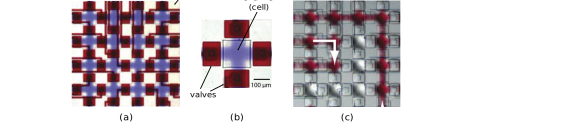
\includegraphics[width=\unitlength,page=1]{archi.pdf}}%
    \put(0.40181094,0.07336126){\color[rgb]{0,0,0}\makebox(0,0)[t]{\lineheight{1.25}\smash{\begin{tabular}[t]{c}valves\end{tabular}}}}%
    \put(0,0){\includegraphics[width=\unitlength,page=2]{archi.pdf}}%
    \put(0.5682774,0.36219924){\color[rgb]{0,0,0}\makebox(0,0)[t]{\lineheight{0}\smash{\begin{tabular}[t]{c}channel\end{tabular}}}}%
    \put(0,0){\includegraphics[width=\unitlength,page=3]{archi.pdf}}%
    \put(0.16168071,0.42865935){\color[rgb]{0,0,0}\makebox(0,0)[t]{\lineheight{0}\smash{\begin{tabular}[t]{c}control\end{tabular}}}}%
    \put(0.16168071,0.40111931){\color[rgb]{0,0,0}\makebox(0,0)[t]{\lineheight{0}\smash{\begin{tabular}[t]{c}channel\end{tabular}}}}%
    \put(0,0){\includegraphics[width=\unitlength,page=4]{archi.pdf}}%
    \put(0.36786319,0.42865935){\color[rgb]{0,0,0}\makebox(0,0)[t]{\lineheight{0}\smash{\begin{tabular}[t]{c}channel\end{tabular}}}}%
    \put(0.36797696,0.40111931){\color[rgb]{0,0,0}\makebox(0,0)[t]{\lineheight{0}\smash{\begin{tabular}[t]{c}wall\end{tabular}}}}%
    \put(0.5678822,0.38968332){\color[rgb]{0,0,0}\makebox(0,0)[t]{\lineheight{0}\smash{\begin{tabular}[t]{c}flow\end{tabular}}}}%
    \put(0.56778639,0.33379743){\color[rgb]{0,0,0}\makebox(0,0)[t]{\lineheight{0}\smash{\begin{tabular}[t]{c}(cell)\end{tabular}}}}%
  \end{picture}%
\endgroup%

\caption{Fully programmable valve array (FPVA) \cite{matrix11}.  (a) Architecture. (b) Valve and cell. (c) Flow path construction. }
\label{fig:archi}
}
\end{figure}

\begin{figure}[t]
{\figurefontsize
\centering
\begingroup%
  \makeatletter%
  \providecommand\color[2][]{%
    \errmessage{(Inkscape) Color is used for the text in Inkscape, but the package 'color.sty' is not loaded}%
    \renewcommand\color[2][]{}%
  }%
  \providecommand\transparent[1]{%
    \errmessage{(Inkscape) Transparency is used (non-zero) for the text in Inkscape, but the package 'transparent.sty' is not loaded}%
    \renewcommand\transparent[1]{}%
  }%
  \providecommand\rotatebox[2]{#2}%
  \newcommand*\fsize{\dimexpr\f@size pt\relax}%
  \newcommand*\lineheight[1]{\fontsize{\fsize}{#1\fsize}\selectfont}%
  \ifx\svgwidth\undefined%
    \setlength{\unitlength}{223.41824396bp}%
    \ifx\svgscale\undefined%
      \relax%
    \else%
      \setlength{\unitlength}{\unitlength * \real{\svgscale}}%
    \fi%
  \else%
    \setlength{\unitlength}{\svgwidth}%
  \fi%
  \global\let\svgwidth\undefined%
  \global\let\svgscale\undefined%
  \makeatother%
  \begin{picture}(1,1.06660424)%
    \lineheight{1}%
    \setlength\tabcolsep{0pt}%
    \put(0.7342614,0.62280321){\color[rgb]{0,0,0}\makebox(0,0)[t]{\lineheight{0}\smash{\begin{tabular}[t]{c}(b)\end{tabular}}}}%
    \put(0.47722094,1.02888716){\color[rgb]{0,0,0}\makebox(0,0)[lt]{\lineheight{0}\smash{\begin{tabular}[t]{l}: closed / wall valves\end{tabular}}}}%
    \put(0,0){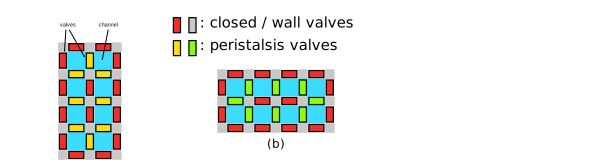
\includegraphics[width=\unitlength,page=1]{dynamic_devices.pdf}}%
    \put(0.17288269,0.84756997){\color[rgb]{0,0,0}\makebox(0,0)[t]{\lineheight{0}\smash{\begin{tabular}[t]{c} \end{tabular}}}}%
    \put(0.10521609,0.53617861){\color[rgb]{0,0,0}\makebox(0,0)[t]{\lineheight{0}\smash{\begin{tabular}[t]{c}(a)\end{tabular}}}}%
    \put(0,0){\includegraphics[width=\unitlength,page=2]{dynamic_devices.pdf}}%
    \put(0.47722094,0.95302425){\color[rgb]{0,0,0}\makebox(0,0)[lt]{\lineheight{0}\smash{\begin{tabular}[t]{l}: peristalsis valves\end{tabular}}}}%
    \put(0,0){\includegraphics[width=\unitlength,page=3]{dynamic_devices.pdf}}%
    \put(0.03357004,1.03151406){\color[rgb]{0,0,0}\makebox(0,0)[t]{\lineheight{0}\smash{\begin{tabular}[t]{c}valves\end{tabular}}}}%
    \put(0,0){\includegraphics[width=\unitlength,page=4]{dynamic_devices.pdf}}%
    \put(0.16852922,1.03185746){\color[rgb]{0,0,0}\makebox(0,0)[t]{\lineheight{1.25}\smash{\begin{tabular}[t]{c}channel\end{tabular}}}}%
    \put(0.19676309,0.00810385){\color[rgb]{0,0,0}\makebox(0,0)[t]{\lineheight{0}\smash{\begin{tabular}[t]{c}(c)\end{tabular}}}}%
    \put(0.71873631,0.00810385){\color[rgb]{0,0,0}\makebox(0,0)[t]{\lineheight{0}\smash{\begin{tabular}[t]{c}(d)\end{tabular}}}}%
    \put(0,0){\includegraphics[width=\unitlength,page=5]{dynamic_devices.pdf}}%
    \put(0.5820626,0.56096611){\color[rgb]{0,0,0}\makebox(0,0)[t]{\lineheight{1.25}\smash{\begin{tabular}[t]{c}no valve\end{tabular}}}}%
    \put(0.81906841,0.51804577){\color[rgb]{0,0,0}\makebox(0,0)[t]{\lineheight{0}\smash{\begin{tabular}[t]{c}always-closed valves\end{tabular}}}}%
    \put(0,0){\includegraphics[width=\unitlength,page=6]{dynamic_devices.pdf}}%
    \put(0.55367855,0.04238681){\color[rgb]{0,0,0}\makebox(0,0)[t]{\lineheight{1.25}\smash{\begin{tabular}[t]{c}1\end{tabular}}}}%
    \put(0.59889592,0.04227309){\color[rgb]{0,0,0}\makebox(0,0)[t]{\lineheight{1.25}\smash{\begin{tabular}[t]{c}2\end{tabular}}}}%
    \put(0.64436173,0.04240873){\color[rgb]{0,0,0}\makebox(0,0)[t]{\lineheight{1.25}\smash{\begin{tabular}[t]{c}3\end{tabular}}}}%
    \put(0.68991328,0.04240873){\color[rgb]{0,0,0}\makebox(0,0)[t]{\lineheight{1.25}\smash{\begin{tabular}[t]{c}4\end{tabular}}}}%
    \put(0.73461381,0.04254416){\color[rgb]{0,0,0}\makebox(0,0)[t]{\lineheight{1.25}\smash{\begin{tabular}[t]{c}5\end{tabular}}}}%
    \put(0.78008228,0.04242184){\color[rgb]{0,0,0}\makebox(0,0)[t]{\lineheight{1.25}\smash{\begin{tabular}[t]{c}6\end{tabular}}}}%
    \put(0.82540477,0.04240873){\color[rgb]{0,0,0}\makebox(0,0)[t]{\lineheight{1.25}\smash{\begin{tabular}[t]{c}7\end{tabular}}}}%
    \put(0.87091247,0.04240873){\color[rgb]{0,0,0}\makebox(0,0)[t]{\lineheight{1.25}\smash{\begin{tabular}[t]{c}8\end{tabular}}}}%
    \put(0.91598909,0.04240422){\color[rgb]{0,0,0}\makebox(0,0)[t]{\lineheight{1.25}\smash{\begin{tabular}[t]{c}9\end{tabular}}}}%
    \put(0.48590842,0.10546882){\color[rgb]{0,0,0}\makebox(0,0)[t]{\lineheight{1.25}\smash{\begin{tabular}[t]{c}1\end{tabular}}}}%
    \put(0.48604826,0.15036718){\color[rgb]{0,0,0}\makebox(0,0)[t]{\lineheight{1.25}\smash{\begin{tabular}[t]{c}2\end{tabular}}}}%
    \put(0.48611382,0.19590276){\color[rgb]{0,0,0}\makebox(0,0)[t]{\lineheight{1.25}\smash{\begin{tabular}[t]{c}3\end{tabular}}}}%
    \put(0.48626677,0.24130105){\color[rgb]{0,0,0}\makebox(0,0)[t]{\lineheight{1.25}\smash{\begin{tabular}[t]{c}4\end{tabular}}}}%
    \put(0.4859871,0.28670487){\color[rgb]{0,0,0}\makebox(0,0)[t]{\lineheight{1.25}\smash{\begin{tabular}[t]{c}5\end{tabular}}}}%
    \put(0.48605696,0.3300979){\color[rgb]{0,0,0}\makebox(0,0)[t]{\lineheight{1.25}\smash{\begin{tabular}[t]{c}6\end{tabular}}}}%
    \put(0.48606137,0.37548513){\color[rgb]{0,0,0}\makebox(0,0)[t]{\lineheight{1.25}\smash{\begin{tabular}[t]{c}7\end{tabular}}}}%
    \put(0.48617068,0.42088322){\color[rgb]{0,0,0}\makebox(0,0)[t]{\lineheight{1.25}\smash{\begin{tabular}[t]{c}8\end{tabular}}}}%
    \put(0.48626677,0.46614751){\color[rgb]{0,0,0}\makebox(0,0)[t]{\lineheight{1.25}\smash{\begin{tabular}[t]{c}9\end{tabular}}}}%
  \end{picture}%
\endgroup%

\caption{FPVA with dynamic devices. (a) A 4$\times$2 dynamic mixer.  (b) A 2$\times$4 dynamic mixer. (c) Dynamic mixers of different orientations sharing the same area. (d) FPVA with a long channel and always-closed valves (obstacles). The x-axis and y-axis show the coordinates of the valves and cells.}
\label{fig:dynamic_devices}
}
\end{figure}


Besides flow paths, devices such as mixers can also be constructed on 
an FPVA, taking advantage of its flexibility and reconfigurability.
For example, a 4$\times$2 mixer and a 2$\times$4 mixer can be constructed as
shown in 
\figname~\ref{fig:dynamic_devices}(a) and \figname~\ref{fig:dynamic_devices}(b),
respectively. In such a dynamic mixer, the eight valves along the enclosed channel 
function as peristalsis valves, which switch in a given pattern 
to drive the fluid segment inside the channel. Compared with the
traditional mixer shown in \figname~\ref{fig:valve_mixer_storage}(b), these dynamic
mixers have different shapes and more peristalsis valves, eight in each case, to
form a 
circular flow for mixing.
Furthermore, the two mixers in 
\figname~\ref{fig:dynamic_devices}(a) and \ref{fig:dynamic_devices}(b)
can share the same chip area as shown in \figname~\ref{fig:dynamic_devices}(c)
if the two mixers are not used at the same time, providing more
flexibility to schedule operations on such a chip.
The videos shown in \cite{PMD_mixing, PMD_transportation} demonstrate
real cases of dynamic device mapping and fluid transportation on an FPVA.

FPVAs have a significant advantage for large-scale integration
due to their regular structure.
The ability of dynamic reconfigurability gives
them the convenience to execute nearly any bioassays, provided specific devices
such as filters and heaters are also built in the chips. 
To facilitate the application of FPVAs, 
the method in \cite{TsengLHS15,TBMTtcad} explores
dynamic mapping of operations to reduce the
maximum number of switching activities of valves, so that valve wearing can be balanced
across all the valves in a chip.
In \cite{pump}, flow routing considering
pressure-routes in establishing transportation paths on an FPVA is investigated
to achieve a better assay completion time. In addition, a
close-to-optimal physical design solution can also be achieved by adapting the
formulation based on satisfiability in \cite{grimmer2017close}.



In the manufacturing process of FPVAs, defects may appear 
at valves and in flow and control channels.
Therefore, 
an efficient design automation method is also required to generate test patterns
for identifying chips with defects. To reduce test cost, the number of these test
patterns should be as small as possible.
In this paper, we address this test generation problem for FPVAs 
with the following contributions:

\begin{itemize}

\item The first systematic formulation of test strategy with test paths and cuts 
  is proposed to enable efficient test of FPVAs after manufacturing.

\item The generation of test patterns
  considers fault masking 
  to cover multiple faults in the flow layer and the control layer.

\item Leakage in control channels is covered by additional test
  paths that are orthogonal to the test paths for stuck-at-0 faults.
  
\item Multiple ports of FPVAs are taken advantage of to improve test
  efficiency. 
  
\item The proposed test framework is completely compatible with existing test
  framework for traditional flow-based biochips,
  so that no additional cost of the test platform is incurred. 
  
\item  When adapted to test traditional biochips, the number of test patterns
  is significantly smaller than that from previously methods based on ATPG, leading
  to a higher test efficiency.

\end{itemize}


The rest of this paper is organized as follows. In
Section~\ref{sec:formulation} we review the state of the art of
testing traditional flow-based biochips and formulate the test problem for FPVAs.
In Section~\ref{sec:test_strategy} we present the general test strategy 
for FPVAs. 
In Section~\ref{sec:path_cut}, the models and their implementation for generating test paths and cuts
are explained in detail.
In Section~\ref{sec:multi_port}, test models are extended to cover biochips
with multiple ports and to adapt the proposed method to test traditional flow-based biochips.
Simulation results are shown in Section~\ref{sec:results} and
conclusions are drawn in Section~\ref{sec:conclusion}.



\section{Fault Model and Problem Formulation}\label{sec:formulation}

During manufacturing of flow-based biochips, various defects may occur. For
example,  the flow channel under a valve may be broken
and does not allow any fluid to pass, leading to a fault equivalent to the
case that the valve cannot be opened. In addition,  leakage may appear between
neighboring flow channels, so that fluids in them may be directed to incorrect
devices or mixed unexpectedly. Furthermore, if the control channel to a valve
becomes broken, air pressure  may not reach the valve. Consequently, this valve
cannot be closed and thus causes a constant leakage.  Furthermore, a leakage may
also appear between two control channels, so that  the valves they drive are
always opened and closed together. 
These cases of manufacturing defects are illustrated 
in \figname~\ref{fig:defects} from \cite{HuYHC14}.



According to how the defects affect the behavior of a valve or a channel,
typical faults 
can be defined as follows:

\begin{itemize}

\item \textit{Broken flow channel}: Fluid cannot pass through a channel. This is
equivalent to the fault that the valve at the entrance of the channel cannot be
opened.  

\item \textit{Leaking flow channel}: Fluid in a channel leaks to its
  neighboring channel. In FPVAs, this fault is similar to the case 
  that a valve separating two cells cannot be closed. 


\item \textit{Broken control channel}: Valve cannot be closed.

\item \textit{Leaking control channel}: Two valves open or close simultaneously
  due to the shared air pressure in the control channels.

\end{itemize}
Since the faults that valves are stuck at the always-closed or always-open
states are similar to the stuck-at-0 faults and stuck-at-1 faults in digital
circuits, these faults are henceforth called \textit{stuck-at-0 faults}
and \textit{stuck-at-1 faults} for convenience.


\begin{figure}[t]
{\figurefontsize
\centering
\begingroup%
  \makeatletter%
  \providecommand\color[2][]{%
    \errmessage{(Inkscape) Color is used for the text in Inkscape, but the package 'color.sty' is not loaded}%
    \renewcommand\color[2][]{}%
  }%
  \providecommand\transparent[1]{%
    \errmessage{(Inkscape) Transparency is used (non-zero) for the text in Inkscape, but the package 'transparent.sty' is not loaded}%
    \renewcommand\transparent[1]{}%
  }%
  \providecommand\rotatebox[2]{#2}%
  \newcommand*\fsize{\dimexpr\f@size pt\relax}%
  \newcommand*\lineheight[1]{\fontsize{\fsize}{#1\fsize}\selectfont}%
  \ifx\svgwidth\undefined%
    \setlength{\unitlength}{225.61093897bp}%
    \ifx\svgscale\undefined%
      \relax%
    \else%
      \setlength{\unitlength}{\unitlength * \real{\svgscale}}%
    \fi%
  \else%
    \setlength{\unitlength}{\svgwidth}%
  \fi%
  \global\let\svgwidth\undefined%
  \global\let\svgscale\undefined%
  \makeatother%
  \begin{picture}(1,0.9140426)%
    \lineheight{1}%
    \setlength\tabcolsep{0pt}%
    \put(0,0){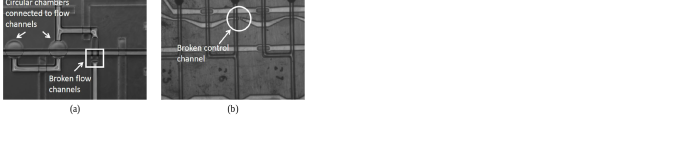
\includegraphics[width=\unitlength,page=1]{defects.pdf}}%
    \put(0.21563204,0.47229537){\color[rgb]{0,0,0}\makebox(0,0)[t]{\lineheight{0}\smash{\begin{tabular}[t]{c}(a)\end{tabular}}}}%
    \put(0,0){\includegraphics[width=\unitlength,page=2]{defects.pdf}}%
    \put(0.75841029,0.47208699){\color[rgb]{0,0,0}\makebox(0,0)[t]{\lineheight{0}\smash{\begin{tabular}[t]{c}(b)\end{tabular}}}}%
    \put(0,0){\includegraphics[width=\unitlength,page=3]{defects.pdf}}%
    \put(0.22785713,0.00657027){\color[rgb]{0,0,0}\makebox(0,0)[t]{\lineheight{0}\smash{\begin{tabular}[t]{c}(c)\end{tabular}}}}%
    \put(0,0){\includegraphics[width=\unitlength,page=4]{defects.pdf}}%
    \put(0.77838155,0.00636209){\color[rgb]{0,0,0}\makebox(0,0)[t]{\lineheight{0}\smash{\begin{tabular}[t]{c}(d)\end{tabular}}}}%
  \end{picture}%
\endgroup%

\caption{Defects in flow-based biochips \cite{HuYHC14}. (a) Broken flow channel. (b) Leaking flow channel. (c) Broken control channel. (d) Leaking control channel.}
\label{fig:defects}
}
\end{figure}

With these fault models, test of traditional flow-based biochips has been
examined in \cite{HuYHC14}. The concept of this method can be explained
using the example illustrated in \figname~\ref{fig:classic_test}(a) from
\cite{HuYHC14}. In this test concept, a pressure source is connected to the
input port of the chip to create air pressure along the channels in the flow
layer. Pressure sensors are attached to the output ports of the chip to detect air
pressure. By switching the valves open or closed according to test patterns,
the air pressure read by the pressure sensors 
at the output ports can be used to determine whether
there is a fault in the chip. In this test process, an air pressure is applied
to the flow channels to detect faults, so that the chip is not
contaminated after test. This air pressure for the purpose of test 
is completely unrelated to the pressure applied in the control channels to 
switch valves when the chip executes bioassays.

In \figname~\ref{fig:classic_test}(a), an air pressure can only be detected at
an output port if there is a path from the pressure source to the output port. For example,
if only the valves $a, g, h, i, k$ are open,  a pressure can be detected
at $o_2$. However, during this test if a valve on this path cannot be opened due to
defects, no pressure can be detected at $o_2$, indicating the
existence of a stuck-at-0 fault. On the other hand, if a valve on this path is also
closed intentionally during the test, all paths from the source to the output
ports should be blocked,
so that no air pressure should be detected at any output port. If, on the
contrary, the test results show that a pressure can still be observed by a
sensor, a stuck-at-1 fault should exist in the chip to allow a path from the
source to an output port to be formed. In this test process,   
the states of the valves during a pressure actuation-measurement cycle is
called a \textit{test pattern}. It is the task of test generation to generate
as few test patterns as possible to detect the faults in a chip efficiently.

To generate test patterns, the method in \cite{HuYHC14} converts the
biochip under test into a circuit as shown in
\figname~\ref{fig:classic_test}(b), where the inputs of the circuit
represent valves and the outputs of the circuit represent the output ports
of the chip. In this circuit representation, valves along the same
channel segment are inputs of AND gates, e.g., $b, c, d, e, f$ and $g,
h$. If two channels converge at a point, 
an OR gate is created in the circuit representation, since a pressure through
any of these channels can reach the converging point. Consequently, 
the circuit represents the relation between valves and the paths from the source to
the output ports in the chip.
To generate test patterns for the biochip, it is
equivalent to generate test patterns for the circuit representation, which can
be achieved by a standard ATPG tool as shown in \cite{HuYHC14}.


The ATPG-based method has the advantage that the biochip under test needs only
to be converted into a circuit representation. The real test generation is
performed using test generation methods for integrated circuits.
However, it is challenging to apply this method directly to test FPVAs
shown in \figname~\ref{fig:archi}(a).  
In converting a biochip into a circuit representation, the structure of the chip
should be known.
On an FPVA, the shapes and locations of devices and transportation
channels are dynamically determined according to the operations to be executed.
If the ATPG-based method is still applied, it then needs to cover 
a huge number of dynamic chip architectures, which is 
a challenging task in view of the flexibility of FPVAs.

\begin{figure}[t]
{\figurefontsize
\centering
\begingroup%
  \makeatletter%
  \providecommand\color[2][]{%
    \errmessage{(Inkscape) Color is used for the text in Inkscape, but the package 'color.sty' is not loaded}%
    \renewcommand\color[2][]{}%
  }%
  \providecommand\transparent[1]{%
    \errmessage{(Inkscape) Transparency is used (non-zero) for the text in Inkscape, but the package 'transparent.sty' is not loaded}%
    \renewcommand\transparent[1]{}%
  }%
  \providecommand\rotatebox[2]{#2}%
  \newcommand*\fsize{\dimexpr\f@size pt\relax}%
  \newcommand*\lineheight[1]{\fontsize{\fsize}{#1\fsize}\selectfont}%
  \ifx\svgwidth\undefined%
    \setlength{\unitlength}{183.91088672bp}%
    \ifx\svgscale\undefined%
      \relax%
    \else%
      \setlength{\unitlength}{\unitlength * \real{\svgscale}}%
    \fi%
  \else%
    \setlength{\unitlength}{\svgwidth}%
  \fi%
  \global\let\svgwidth\undefined%
  \global\let\svgscale\undefined%
  \makeatother%
  \begin{picture}(1,0.7370509)%
    \lineheight{1}%
    \setlength\tabcolsep{0pt}%
    \put(0,0){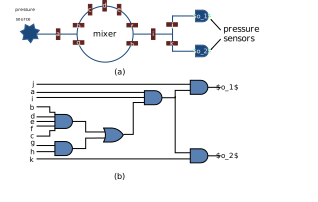
\includegraphics[width=\unitlength,page=1]{ref_test_biochip.pdf}}%
    \put(0.30335142,0.69036144){\color[rgb]{1,1,1}\makebox(0,0)[t]{\lineheight{0}\smash{\begin{tabular}[t]{c}c\end{tabular}}}}%
    \put(0,0){\includegraphics[width=\unitlength,page=2]{ref_test_biochip.pdf}}%
    \put(0.3625445,0.7063789){\color[rgb]{1,1,1}\makebox(0,0)[t]{\lineheight{0}\smash{\begin{tabular}[t]{c}d\end{tabular}}}}%
    \put(0,0){\includegraphics[width=\unitlength,page=3]{ref_test_biochip.pdf}}%
    \put(0.42173764,0.69036144){\color[rgb]{1,1,1}\makebox(0,0)[t]{\lineheight{0}\smash{\begin{tabular}[t]{c}e\end{tabular}}}}%
    \put(0,0){\includegraphics[width=\unitlength,page=4]{ref_test_biochip.pdf}}%
    \put(0.25655341,0.6224595){\color[rgb]{1,1,1}\makebox(0,0)[t]{\lineheight{0}\smash{\begin{tabular}[t]{c}b\end{tabular}}}}%
    \put(0,0){\includegraphics[width=\unitlength,page=5]{ref_test_biochip.pdf}}%
    \put(0.25655341,0.55573662){\color[rgb]{1,1,1}\makebox(0,0)[t]{\lineheight{0}\smash{\begin{tabular}[t]{c}g\end{tabular}}}}%
    \put(0,0){\includegraphics[width=\unitlength,page=6]{ref_test_biochip.pdf}}%
    \put(0.47553814,0.61831844){\color[rgb]{1,1,1}\makebox(0,0)[t]{\lineheight{0}\smash{\begin{tabular}[t]{c}f\end{tabular}}}}%
    \put(0,0){\includegraphics[width=\unitlength,page=7]{ref_test_biochip.pdf}}%
    \put(0.47553814,0.54628108){\color[rgb]{1,1,1}\makebox(0,0)[t]{\lineheight{0}\smash{\begin{tabular}[t]{c}h\end{tabular}}}}%
    \put(0,0){\includegraphics[width=\unitlength,page=8]{ref_test_biochip.pdf}}%
    \put(0.17281526,0.59033947){\color[rgb]{1,1,1}\makebox(0,0)[t]{\lineheight{0}\smash{\begin{tabular}[t]{c}a\end{tabular}}}}%
    \put(0,0){\includegraphics[width=\unitlength,page=9]{ref_test_biochip.pdf}}%
    \put(0.56100453,0.59033947){\color[rgb]{1,1,1}\makebox(0,0)[t]{\lineheight{0}\smash{\begin{tabular}[t]{c}i\end{tabular}}}}%
    \put(0,0){\includegraphics[width=\unitlength,page=10]{ref_test_biochip.pdf}}%
    \put(0.63822853,0.62623866){\color[rgb]{1,1,1}\makebox(0,0)[t]{\lineheight{0}\smash{\begin{tabular}[t]{c}j\end{tabular}}}}%
    \put(0,0){\includegraphics[width=\unitlength,page=11]{ref_test_biochip.pdf}}%
    \put(0.63822853,0.55137869){\color[rgb]{1,1,1}\makebox(0,0)[t]{\lineheight{0}\smash{\begin{tabular}[t]{c}k\end{tabular}}}}%
    \put(0,0){\includegraphics[width=\unitlength,page=12]{ref_test_biochip.pdf}}%
    \put(-0.00158789,0.69234335){\color[rgb]{0,0,0}\makebox(0,0)[lt]{\lineheight{0}\smash{\begin{tabular}[t]{l}pressure \end{tabular}}}}%
    \put(-0.0003241,0.6536972){\color[rgb]{0,0,0}\makebox(0,0)[lt]{\lineheight{0}\smash{\begin{tabular}[t]{l}source\end{tabular}}}}%
    \put(0,0){\includegraphics[width=\unitlength,page=13]{ref_test_biochip.pdf}}%
    \put(0.76060006,0.51949584){\color[rgb]{1,1,1}\makebox(0,0)[t]{\lineheight{0}\smash{\begin{tabular}[t]{c}$o_2$\end{tabular}}}}%
    \put(0.31587142,0.58773534){\color[rgb]{0,0,0}\makebox(0,0)[lt]{\lineheight{0}\smash{\begin{tabular}[t]{l}mixer\end{tabular}}}}%
    \put(0,0){\includegraphics[width=\unitlength,page=14]{ref_test_biochip.pdf}}%
    \put(0.84721895,0.60740523){\color[rgb]{0,0,0}\makebox(0,0)[lt]{\lineheight{0}\smash{\begin{tabular}[t]{l}pressure \end{tabular}}}}%
    \put(0.84848279,0.56875908){\color[rgb]{0,0,0}\makebox(0,0)[lt]{\lineheight{0}\smash{\begin{tabular}[t]{l}sensors\end{tabular}}}}%
    \put(0.76060006,0.66231447){\color[rgb]{1,1,1}\makebox(0,0)[t]{\lineheight{0}\smash{\begin{tabular}[t]{c}$o_1$\end{tabular}}}}%
    \put(0,0){\includegraphics[width=\unitlength,page=15]{ref_test_biochip.pdf}}%
    \put(0.06733809,0.17296396){\color[rgb]{0,0,0}\makebox(0,0)[t]{\lineheight{0}\smash{\begin{tabular}[t]{c}c\end{tabular}}}}%
    \put(0.06822243,0.25280406){\color[rgb]{0,0,0}\makebox(0,0)[t]{\lineheight{0}\smash{\begin{tabular}[t]{c}d\end{tabular}}}}%
    \put(0.06763522,0.23059059){\color[rgb]{0,0,0}\makebox(0,0)[t]{\lineheight{0}\smash{\begin{tabular}[t]{c}e\end{tabular}}}}%
    \put(0.06713295,0.28871955){\color[rgb]{0,0,0}\makebox(0,0)[t]{\lineheight{0}\smash{\begin{tabular}[t]{c}b\end{tabular}}}}%
    \put(0.06822243,0.14571584){\color[rgb]{0,0,0}\makebox(0,0)[t]{\lineheight{0}\smash{\begin{tabular}[t]{c}g\end{tabular}}}}%
    \put(0.06672966,0.20104251){\color[rgb]{0,0,0}\makebox(0,0)[t]{\lineheight{0}\smash{\begin{tabular}[t]{c}f\end{tabular}}}}%
    \put(0.06762109,0.10716967){\color[rgb]{0,0,0}\makebox(0,0)[t]{\lineheight{0}\smash{\begin{tabular}[t]{c}h\end{tabular}}}}%
    \put(0.0682083,0.35328228){\color[rgb]{0,0,0}\makebox(0,0)[t]{\lineheight{0}\smash{\begin{tabular}[t]{c}a\end{tabular}}}}%
    \put(0.06769185,0.32327734){\color[rgb]{0,0,0}\makebox(0,0)[t]{\lineheight{0}\smash{\begin{tabular}[t]{c}i\end{tabular}}}}%
    \put(0.06932609,0.38527859){\color[rgb]{0,0,0}\makebox(0,0)[t]{\lineheight{0}\smash{\begin{tabular}[t]{c}j\end{tabular}}}}%
    \put(0.06640422,0.07586297){\color[rgb]{0,0,0}\makebox(0,0)[t]{\lineheight{0}\smash{\begin{tabular}[t]{c}k\end{tabular}}}}%
    \put(0.86188074,0.09227412){\color[rgb]{0,0,0}\makebox(0,0)[t]{\lineheight{0}\smash{\begin{tabular}[t]{c}$o_2$\end{tabular}}}}%
    \put(0.86188074,0.37180712){\color[rgb]{0,0,0}\makebox(0,0)[t]{\lineheight{0}\smash{\begin{tabular}[t]{c}$o_1$\end{tabular}}}}%
    \put(0.40175302,0.43282083){\color[rgb]{0,0,0}\makebox(0,0)[lt]{\lineheight{0}\smash{\begin{tabular}[t]{l}(a)\end{tabular}}}}%
    \put(0.40139816,0.00664599){\color[rgb]{0,0,0}\makebox(0,0)[lt]{\lineheight{0}\smash{\begin{tabular}[t]{l}(b)\end{tabular}}}}%
    \put(0.63822853,0.62419961){\color[rgb]{1,1,1}\makebox(0,0)[t]{\lineheight{0}\smash{\begin{tabular}[t]{c}j\end{tabular}}}}%
  \end{picture}%
\endgroup%

\caption{Test of traditional flow-based biochips \cite{HuYHC14}. (a) Schematic of the chip under test. (b) Circuit representation of the test model for test pattern generation.}
\label{fig:classic_test}
}
\end{figure}

In this paper, we propose a new test framework for detecting faults in an FPVA
with only a small set of test patterns. This problem can be formulated as follows:
\begin{itemize}

  \item{Input:} An FPVA architecture; the locations of long channels (no valve
    built, conceptually always open) and obstacles (conceptually always
    closed); the locations of the air pressure source and the pressure sensors.

\item{Output:} A set of test patterns, each of which defines the
open/closed states of all valves when test pressure is applied
at the source and checked at the output ports by the pressure sensors.

\item{Objective:} The number of test patterns should be 
  as small as possible to reduce test cost; faults should be detected reliably by
  covering all valves.

\end{itemize}


\begin{figure}[t]
{\figurefontsize
\centering
\begingroup%
  \makeatletter%
  \providecommand\color[2][]{%
    \errmessage{(Inkscape) Color is used for the text in Inkscape, but the package 'color.sty' is not loaded}%
    \renewcommand\color[2][]{}%
  }%
  \providecommand\transparent[1]{%
    \errmessage{(Inkscape) Transparency is used (non-zero) for the text in Inkscape, but the package 'transparent.sty' is not loaded}%
    \renewcommand\transparent[1]{}%
  }%
  \providecommand\rotatebox[2]{#2}%
  \newcommand*\fsize{\dimexpr\f@size pt\relax}%
  \newcommand*\lineheight[1]{\fontsize{\fsize}{#1\fsize}\selectfont}%
  \ifx\svgwidth\undefined%
    \setlength{\unitlength}{257.44990564bp}%
    \ifx\svgscale\undefined%
      \relax%
    \else%
      \setlength{\unitlength}{\unitlength * \real{\svgscale}}%
    \fi%
  \else%
    \setlength{\unitlength}{\svgwidth}%
  \fi%
  \global\let\svgwidth\undefined%
  \global\let\svgscale\undefined%
  \makeatother%
  \begin{picture}(1,1.00777318)%
    \lineheight{1}%
    \setlength\tabcolsep{0pt}%
    \put(0,0){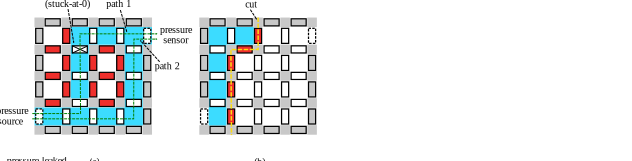
\includegraphics[width=\unitlength,page=1]{path_cutset.pdf}}%
    \put(0.52668259,0.88237203){\color[rgb]{0,0,0}\makebox(0,0)[t]{\lineheight{0}\smash{\begin{tabular}[t]{c}pressure\end{tabular}}}}%
    \put(0.52571585,0.85227999){\color[rgb]{0,0,0}\makebox(0,0)[t]{\lineheight{0}\smash{\begin{tabular}[t]{c}sensor\end{tabular}}}}%
    \put(0.00009957,0.64591962){\color[rgb]{0,0,0}\makebox(0,0)[lt]{\lineheight{0}\smash{\begin{tabular}[t]{l}pressure\end{tabular}}}}%
    \put(0.00444935,0.6152458){\color[rgb]{0,0,0}\makebox(0,0)[lt]{\lineheight{0}\smash{\begin{tabular}[t]{l}source\end{tabular}}}}%
    \put(0,0){\includegraphics[width=\unitlength,page=2]{path_cutset.pdf}}%
    \put(0.20421121,0.98754587){\color[rgb]{0,0,0}\makebox(0,0)[t]{\lineheight{0}\smash{\begin{tabular}[t]{c}valve under test\end{tabular}}}}%
    \put(0,0){\includegraphics[width=\unitlength,page=3]{path_cutset.pdf}}%
    \put(0.35809036,0.95820685){\color[rgb]{0,0,0}\makebox(0,0)[t]{\lineheight{0}\smash{\begin{tabular}[t]{c}path 1\end{tabular}}}}%
    \put(0.49969542,0.77663721){\color[rgb]{0,0,0}\makebox(0,0)[t]{\lineheight{0}\smash{\begin{tabular}[t]{c}path 2\end{tabular}}}}%
    \put(0,0){\includegraphics[width=\unitlength,page=4]{path_cutset.pdf}}%
    \put(0.74451826,0.95674883){\color[rgb]{0,0,0}\makebox(0,0)[t]{\lineheight{0}\smash{\begin{tabular}[t]{c}cut\end{tabular}}}}%
    \put(0,0){\includegraphics[width=\unitlength,page=5]{path_cutset.pdf}}%
    \put(0.28690947,0.49637158){\color[rgb]{0,0,0}\makebox(0,0)[t]{\lineheight{0}\smash{\begin{tabular}[t]{c}(a)\end{tabular}}}}%
    \put(0.76974034,0.49637158){\color[rgb]{0,0,0}\makebox(0,0)[t]{\lineheight{0}\smash{\begin{tabular}[t]{c}(b)\end{tabular}}}}%
    \put(0,0){\includegraphics[width=\unitlength,page=6]{path_cutset.pdf}}%
    \put(0.20828797,0.95820685){\color[rgb]{0,0,0}\makebox(0,0)[t]{\lineheight{0}\smash{\begin{tabular}[t]{c}(stuck-at-0)\end{tabular}}}}%
    \put(0,0){\includegraphics[width=\unitlength,page=7]{path_cutset.pdf}}%
    \put(0.49672231,0.27987836){\color[rgb]{0,0,0}\makebox(0,0)[t]{\lineheight{0}\smash{\begin{tabular}[t]{c}test\end{tabular}}}}%
    \put(0,0){\includegraphics[width=\unitlength,page=8]{path_cutset.pdf}}%
    \put(0.35953291,0.06074719){\color[rgb]{0,0,0}\makebox(0,0)[t]{\lineheight{0}\smash{\begin{tabular}[t]{c}valve cannot open\end{tabular}}}}%
    \put(0.28198173,0.00623035){\color[rgb]{0,0,0}\makebox(0,0)[t]{\lineheight{0}\smash{\begin{tabular}[t]{c}(c)\end{tabular}}}}%
    \put(0.49774203,0.25103275){\color[rgb]{0,0,0}\makebox(0,0)[t]{\lineheight{0}\smash{\begin{tabular}[t]{c}path\end{tabular}}}}%
    \put(0.11676614,0.05783116){\color[rgb]{0,0,0}\makebox(0,0)[t]{\lineheight{0}\smash{\begin{tabular}[t]{c}valve cannot close\end{tabular}}}}%
    \put(0.36397293,0.0266481){\color[rgb]{0,0,0}\makebox(0,0)[t]{\lineheight{0}\smash{\begin{tabular}[t]{c}(valve 1)\end{tabular}}}}%
    \put(0.11933776,0.0266481){\color[rgb]{0,0,0}\makebox(0,0)[t]{\lineheight{0}\smash{\begin{tabular}[t]{c}(valve 2)\end{tabular}}}}%
    \put(0,0){\includegraphics[width=\unitlength,page=9]{path_cutset.pdf}}%
    \put(0.74240902,0.4666076){\color[rgb]{0,0,0}\makebox(0,0)[t]{\lineheight{0}\smash{\begin{tabular}[t]{c}cut\end{tabular}}}}%
    \put(0,0){\includegraphics[width=\unitlength,page=10]{path_cutset.pdf}}%
    \put(0.63390859,0.06074719){\color[rgb]{0,0,0}\makebox(0,0)[t]{\lineheight{0}\smash{\begin{tabular}[t]{c}leaked pressure   \end{tabular}}}}%
    \put(0,0){\includegraphics[width=\unitlength,page=11]{path_cutset.pdf}}%
    \put(0.76683436,0.00623035){\color[rgb]{0,0,0}\makebox(0,0)[t]{\lineheight{0}\smash{\begin{tabular}[t]{c}(d)\end{tabular}}}}%
    \put(0,0){\includegraphics[width=\unitlength,page=12]{path_cutset.pdf}}%
    \put(0.81491014,0.23029762){\color[rgb]{0,0,0}\makebox(0,0)[t]{\lineheight{0}\smash{\begin{tabular}[t]{c}$c_{i_1,j_1}^m$\end{tabular}}}}%
    \put(0.86582977,0.06275676){\color[rgb]{0,0,0}\makebox(0,0)[t]{\lineheight{0}\smash{\begin{tabular}[t]{c}$c_{i_2,j_2}^m$\end{tabular}}}}%
    \put(0.92846473,0.07194067){\color[rgb]{0,0,0}\makebox(0,0)[t]{\lineheight{0}\smash{\begin{tabular}[t]{c}$v_{i,j}^m$\end{tabular}}}}%
    \put(0.63257753,0.02667655){\color[rgb]{0,0,0}\makebox(0,0)[t]{\lineheight{0}\smash{\begin{tabular}[t]{c}blocked by valve 1\end{tabular}}}}%
    \put(0,0){\includegraphics[width=\unitlength,page=13]{path_cutset.pdf}}%
    \put(0.11856839,0.50032067){\color[rgb]{0,0,0}\makebox(0,0)[t]{\lineheight{0}\smash{\begin{tabular}[t]{c}pressure leaked\end{tabular}}}}%
    \put(0.12303775,0.46809406){\color[rgb]{0,0,0}\makebox(0,0)[t]{\lineheight{0}\smash{\begin{tabular}[t]{c}through valve 2\end{tabular}}}}%
  \end{picture}%
\endgroup%

\caption{Flow paths and cuts. Valves at the external boundary of the chip are always closed. (a) Test paths and stuck-at-0 fault masking. (b) Cut.  (c) Test path with two-fault masking. (d) Cut with two-fault masking and variables to prevent fault masking.}
\label{fig:path_cutset}
}
\end{figure}


\section{Flow paths and cuts for FPVA test} %
\label{sec:test_strategy}

In the test process, the open/closed states of valves in an FPVA are set
according to test patterns,
and the pressure values at the output ports are measured by 
pressure sensors. Faults can thus be detected by comparing the readout
with expected values.


To identify whether faults exist in a chip, a test pattern should ensure
that faults are observable by the pressure sensors at the output ports.
For example, faults caused by valves that cannot be opened, stuck-at-0 faults, 
can be detected by creating paths from the pressure source to the pressure
sensors. If, however, no pressure sensors can read a valid pressure value at
the outputs, some valves on the path should have defects, and cannot
be opened by the test pattern to allow the test pressure to pass. 
Similarly, if a test pattern 
cuts off all the paths 
from the pressure source to the pressure sensors but 
the sensors still detect pressure valves, 
stuck-at-1 faults allowing pressure leakage at valves must exist in the chip.
\figname~\ref{fig:path_cutset}(a) and \ref{fig:path_cutset}(b) 
illustrate the concepts of test patterns to
test stuck-at-0 and stuck-at-1 faults.

When test patterns are applied, some faults might mask each other. For
example, two test paths are created in the FPVA illustrated in
\figname~\ref{fig:path_cutset}(a) simultaneously. If a valve on one of the paths is defected, the
air pressure can still reach the pressure sensor through the other path.
Therefore, this stuck-at-0 fault cannot be observed at the output port.
To avoid this path interference problem, only simple paths without loops should
be constructed. These paths are called \textit{test paths} henceforth.
Similar to test paths,
test cuts can be constructed to detect stuck-at-1 faults. 
A \textit{test cut}
is formed by a set of valves that separate the pressure source and the pressure
sensors completely when they are closed, so that no test pressure can reach
the sensors, as illustrated in \figname~\ref{fig:path_cutset}(b).


\begin{figure*}[t]
{\figurefontsize
\centering
\begingroup%
  \makeatletter%
  \providecommand\color[2][]{%
    \errmessage{(Inkscape) Color is used for the text in Inkscape, but the package 'color.sty' is not loaded}%
    \renewcommand\color[2][]{}%
  }%
  \providecommand\transparent[1]{%
    \errmessage{(Inkscape) Transparency is used (non-zero) for the text in Inkscape, but the package 'transparent.sty' is not loaded}%
    \renewcommand\transparent[1]{}%
  }%
  \providecommand\rotatebox[2]{#2}%
  \newcommand*\fsize{\dimexpr\f@size pt\relax}%
  \newcommand*\lineheight[1]{\fontsize{\fsize}{#1\fsize}\selectfont}%
  \ifx\svgwidth\undefined%
    \setlength{\unitlength}{501.98811865bp}%
    \ifx\svgscale\undefined%
      \relax%
    \else%
      \setlength{\unitlength}{\unitlength * \real{\svgscale}}%
    \fi%
  \else%
    \setlength{\unitlength}{\svgwidth}%
  \fi%
  \global\let\svgwidth\undefined%
  \global\let\svgscale\undefined%
  \makeatother%
  \begin{picture}(1,0.24722313)%
    \lineheight{1}%
    \setlength\tabcolsep{0pt}%
    \put(0,0){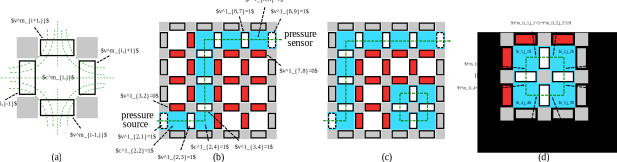
\includegraphics[width=\unitlength,page=1]{flow_path_model.pdf}}%
    \put(0.07466184,0.20939855){\color[rgb]{0,0,0}\makebox(0,0)[t]{\lineheight{0}\smash{\begin{tabular}[t]{c} $v^m_{i+1,j}$\end{tabular}}}}%
    \put(0.16223907,0.03849428){\color[rgb]{0,0,0}\makebox(0,0)[t]{\lineheight{0}\smash{\begin{tabular}[t]{c} $v^m_{i-1,j}$\end{tabular}}}}%
    \put(0.02732203,0.08519193){\color[rgb]{0,0,0}\makebox(0,0)[t]{\lineheight{0}\smash{\begin{tabular}[t]{c} $v^m_{i,j-1}$\end{tabular}}}}%
    \put(0.20888119,0.16425542){\color[rgb]{0,0,0}\makebox(0,0)[t]{\lineheight{0}\smash{\begin{tabular}[t]{c} $v^m_{i,j+1}$\end{tabular}}}}%
    \put(0.1167175,0.12421848){\color[rgb]{0,0,0}\makebox(0,0)[t]{\lineheight{0}\smash{\begin{tabular}[t]{c} $c^m_{i,j}$\end{tabular}}}}%
    \put(0.74426438,0.19486467){\color[rgb]{0,0,0}\makebox(0,0)[lt]{\begin{minipage}{0.2250259\unitlength}\centering  \end{minipage}}}%
    \put(0.11411867,0.00324755){\color[rgb]{0,0,0}\makebox(0,0)[t]{\lineheight{0}\smash{\begin{tabular}[t]{c}(a)\end{tabular}}}}%
    \put(0.23479095,0.03573213){\color[rgb]{0,0,0}\makebox(0,0)[t]{\lineheight{0}\smash{\begin{tabular}[t]{c} $v^1_{2,1}=1$\end{tabular}}}}%
    \put(0.23112447,0.01464194){\color[rgb]{0,0,0}\makebox(0,0)[t]{\lineheight{0}\smash{\begin{tabular}[t]{c} $c^1_{2,2}=1$\end{tabular}}}}%
    \put(0,0){\includegraphics[width=\unitlength,page=2]{flow_path_model.pdf}}%
    \put(0.47988729,0.18757502){\color[rgb]{0,0,0}\makebox(0,0)[t]{\lineheight{0}\smash{\begin{tabular}[t]{c}pressure\end{tabular}}}}%
    \put(0.47939149,0.17425488){\color[rgb]{0,0,0}\makebox(0,0)[t]{\lineheight{0}\smash{\begin{tabular}[t]{c}sensor\end{tabular}}}}%
    \put(0.21109423,0.06618444){\color[rgb]{0,0,0}\makebox(0,0)[lt]{\lineheight{0}\smash{\begin{tabular}[t]{l}pressure\end{tabular}}}}%
    \put(0.21332506,0.05256601){\color[rgb]{0,0,0}\makebox(0,0)[lt]{\lineheight{0}\smash{\begin{tabular}[t]{l}source\end{tabular}}}}%
    \put(0,0){\includegraphics[width=\unitlength,page=3]{flow_path_model.pdf}}%
    \put(0.35665285,0.0031953){\color[rgb]{0,0,0}\makebox(0,0)[t]{\lineheight{0}\smash{\begin{tabular}[t]{c}(b)\end{tabular}}}}%
    \put(0,0){\includegraphics[width=\unitlength,page=4]{flow_path_model.pdf}}%
    \put(0.29415113,0.00489445){\color[rgb]{0,0,0}\makebox(0,0)[t]{\lineheight{0}\smash{\begin{tabular}[t]{c} $v^1_{2,3}=1$\end{tabular}}}}%
    \put(0,0){\includegraphics[width=\unitlength,page=5]{flow_path_model.pdf}}%
    \put(0.4093913,0.02047866){\color[rgb]{0,0,0}\makebox(0,0)[t]{\lineheight{0}\smash{\begin{tabular}[t]{c} $v^1_{3,4}=1$\end{tabular}}}}%
    \put(0,0){\includegraphics[width=\unitlength,page=6]{flow_path_model.pdf}}%
    \put(0.34344779,0.02047866){\color[rgb]{0,0,0}\makebox(0,0)[t]{\lineheight{0}\smash{\begin{tabular}[t]{c} $c^1_{2,4}=1$\end{tabular}}}}%
    \put(0,0){\includegraphics[width=\unitlength,page=7]{flow_path_model.pdf}}%
    \put(0.46320451,0.22303412){\color[rgb]{0,0,0}\makebox(0,0)[t]{\lineheight{0}\smash{\begin{tabular}[t]{c} $v^1_{8,9}=1$\end{tabular}}}}%
    \put(0.38140477,0.22303412){\color[rgb]{0,0,0}\makebox(0,0)[t]{\lineheight{0}\smash{\begin{tabular}[t]{c} $v^1_{8,7}=1$\end{tabular}}}}%
    \put(0.47627753,0.13412483){\color[rgb]{0,0,0}\makebox(0,0)[t]{\lineheight{0}\smash{\begin{tabular}[t]{c} $v^1_{7,8}=0$\end{tabular}}}}%
    \put(0.42531984,0.24078875){\color[rgb]{0,0,0}\makebox(0,0)[t]{\lineheight{0}\smash{\begin{tabular}[t]{c} $c^1_{8,8}=1$\end{tabular}}}}%
    \put(0,0){\includegraphics[width=\unitlength,page=8]{flow_path_model.pdf}}%
    \put(0.23841261,0.09652239){\color[rgb]{0,0,0}\makebox(0,0)[t]{\lineheight{0}\smash{\begin{tabular}[t]{c} $v^1_{3,2}=0$\end{tabular}}}}%
    \put(0,0){\includegraphics[width=\unitlength,page=9]{flow_path_model.pdf}}%
    \put(0.60849977,0.00324755){\color[rgb]{0,0,0}\makebox(0,0)[t]{\lineheight{0}\smash{\begin{tabular}[t]{c}(c)\end{tabular}}}}%
    \put(0,0){\includegraphics[width=\unitlength,page=10]{flow_path_model.pdf}}%
    \put(0.84356671,0.0031953){\color[rgb]{0,0,0}\makebox(0,0)[t]{\lineheight{0}\smash{\begin{tabular}[t]{c}(d)\end{tabular}}}}%
    \put(0,0){\includegraphics[width=\unitlength,page=11]{flow_path_model.pdf}}%
    \put(0.81301938,0.16396088){\color[rgb]{0,0,0}\makebox(0,0)[t]{\lineheight{0}\smash{\begin{tabular}[t]{c}$i_1,j_1$\end{tabular}}}}%
    \put(0.83954185,0.20655999){\color[rgb]{0,0,0}\makebox(0,0)[t]{\lineheight{0}\smash{\begin{tabular}[t]{c}  $-f^m_{i_1,j_1+1}=f^m_{i_2,j_2-1}$\end{tabular}}}}%
    \put(0,0){\includegraphics[width=\unitlength,page=12]{flow_path_model.pdf}}%
    \put(0.85687381,0.04696493){\color[rgb]{0,0,0}\makebox(0,0)[t]{\lineheight{0}\smash{\begin{tabular}[t]{c}  $f^m_{i_4,j_4+1}=-f^m_{i_3,j_3-1}$\end{tabular}}}}%
    \put(0,0){\includegraphics[width=\unitlength,page=13]{flow_path_model.pdf}}%
    \put(0.94687866,0.10890966){\color[rgb]{0,0,0}\makebox(0,0)[t]{\lineheight{0}\smash{\begin{tabular}[t]{c}  $f^m_{i_3+1,j_3}$\end{tabular}}}}%
    \put(0.94973528,0.14275114){\color[rgb]{0,0,0}\makebox(0,0)[t]{\lineheight{0}\smash{\begin{tabular}[t]{c}$-f^m_{i_2-1,j_2}$\end{tabular}}}}%
    \put(0.94297016,0.12706598){\color[rgb]{0,0,0}\rotatebox{-90}{\makebox(0,0)[t]{\lineheight{0}\smash{\begin{tabular}[t]{c}=\end{tabular}}}}}%
    \put(0,0){\includegraphics[width=\unitlength,page=14]{flow_path_model.pdf}}%
    \put(0.73804713,0.10949702){\color[rgb]{0,0,0}\makebox(0,0)[t]{\lineheight{0}\smash{\begin{tabular}[t]{c} $-f^m_{i_4+1,j_4}$\end{tabular}}}}%
    \put(0.74720408,0.14518711){\color[rgb]{0,0,0}\makebox(0,0)[t]{\lineheight{0}\smash{\begin{tabular}[t]{c}$f^m_{i_1-1,j_1}$\end{tabular}}}}%
    \put(0.73712675,0.12950195){\color[rgb]{0,0,0}\rotatebox{-90}{\makebox(0,0)[t]{\lineheight{0}\smash{\begin{tabular}[t]{c}=\end{tabular}}}}}%
    \put(0.87714474,0.16396088){\color[rgb]{0,0,0}\makebox(0,0)[t]{\lineheight{0}\smash{\begin{tabular}[t]{c}$i_2,j_2$\end{tabular}}}}%
    \put(0.87714474,0.08750469){\color[rgb]{0,0,0}\makebox(0,0)[t]{\lineheight{0}\smash{\begin{tabular}[t]{c}$i_3,j_3$\end{tabular}}}}%
    \put(0.81301938,0.08750469){\color[rgb]{0,0,0}\makebox(0,0)[t]{\lineheight{0}\smash{\begin{tabular}[t]{c}$i_4,j_4$\end{tabular}}}}%
    \put(0,0){\includegraphics[width=\unitlength,page=15]{flow_path_model.pdf}}%
  \end{picture}%
\endgroup%

\caption{Flow path model. (a) Constraint variables for valves and cells. (b) Path construction using constraints. (c) Disjoint loop. (d) Flow constraints along a disjoint loop.}
\label{fig:flow_path_model}
}
\end{figure*}

Based on the analysis above, the test patterns that need to be constructed for
testing an FPVA can be defined as follows:

\begin{itemize} 
 
  \item\textit{Test-path patterns}: A set of paths between the pressure source
    and the pressure sensors. These paths should cover each valve at least once. 
    A test path should be a simple
path without a loop, so that no parallel path segment
that can mask stuck-at-0 faults is present. A test path is thus
similar to a ``self-avoiding walk'' on a lattice, which is well studied
elsewhere in the context of grid graphs \cite{walk1996}.
    In the test
    process, test paths are applied one after another, in each of which only
    the valves on the path are opened and all the other valves are closed.
    If no test pressure is detected, 
    stuck-at-0 fault should exist.
 
\item\textit{Test-cut patterns}:  A set of cuts, each of which is formed from a
  series of valves 
  separating the pressure source and the pressure sensors 
  completely when they are closed. The generated cuts should cover each valve at least once to test
  whether it can be closed. When a cut is applied but air pressure is still
  detected by a sensor, at least a valve in the cut should have stuck-at-1 fault. 
\end{itemize}

The path and cut test patterns can detect any single fault in the chip. 
If multiple faults exist, fault masking might still happen.
Assume that there are two faulty valves, one of which cannot be opened (valve
1, stuck-at-0) and the other cannot be closed (valve 2, stuck-at-1).  Also
assume that the test path used to test valve 1 is constructed as shown in  
\figname~\ref{fig:path_cutset}(c), and  the cut used to test valve 2 is
constructed as shown  in \figname~\ref{fig:path_cutset}(d). In 
\figname~\ref{fig:path_cutset}(c), the test pressure can still bypass the
broken valve 1 and reach the pressure sensor though valve 2. In other words,
the pressure leakage through valve 2 masks the stuck-at-0 fault at valve 1. 
In \figname~\ref{fig:path_cutset}(d), the
pressure leakage through valve 2 is blocked by valve 1, 
so that no test pressure can reach the sensor,
leading to mutual masking of faulty valves.
Consequently, none of these faulty valves can be detected by the test patterns. 
To solve this problem, such mutual masking
cases should be excluded from the generated test patterns. 





\section{Generating test-path and test-cut patterns} 
\label{sec:path_cut}

The objective of generating path and cut test patterns is
to minimize the number of test patterns to reduce test cost. The path patterns
together should cover all valves to detect stuck-at-0 faults, and so  
are the cut patterns to detect stuck-at-1 faults. Furthermore, leakage in
control layers causes two valves to switch simultaneously, so that such faults
should also be covered by the test patterns. The test patterns described in
this section assume that there is a single pressure source and a single
pressure sensor for fault test. Test patterns with multiple sensors will be discussed in
Section~\ref{sec:multi_port}.


\subsection{Constructing path test patterns} 
\label{sec:flow_paths}

In an FPVA, a test path can pass through a valve from any of the two
directions.  
The test paths together should cover each valve in the chip at least once.
In the proposed method, we describe this path generation using an Integer Linear
Programming (ILP) model.  The scalability of this model is further improved
using a heuristic loop removal technique. 

\subsubsection{Path pattern formulation} \label{sec:flow_path_cons}

In an FPVA, a fluid cell is defined as the channel area surrounded by four
valves. A test path can enter such a   
cell and leave it from any of the four valves surrounding the cell.
Consequently,  
there are 12 possible directions for a path passing through a cell, 
as illustrated by the dashed lines in \figname~\ref{fig:flow_path_model}(a).

In describing the path model, a valve
and a fluid cell in an FPVA are denoted as $\mathtt{V}_{i,}$ and
$\mathtt{C}_{i,j}$, respectively, where $(i,j)$ is the coordinate as shown in
\figname~\ref{fig:dynamic_devices}(d).
Assume all valves can be covered by 
no more than $n_p$ test paths, 
where $n_p$ is a given constant. 
For the cell at the location $(i,j)$, we assign
a 0-1 variable $c^m_{i,j}$ to represent whether the $m$th path travels through
the cell. If the $m$th path travels through the cell,
$c^m_{i,j}=1$; otherwise $c^m_{i,j}=0$.
For the valves at the left, right, upper and lower sides of the cell, 
we assign 0-1 variables 
$v_{i, j-1}^m$, $v_{i, j+1}^m$, $v_{i+1, j}^m$ and, $v_{i-1, j}^m$, respectively. If 
the $m$th path travels through a valve, the corresponding variable is set to 1;
otherwise, it is set to 0.  

If the $m$th path travels through
the cell $\mathtt{C}_{i,j}$ at the location $(i,j)$, this path should travel through exactly 
two valves that surround the cell.
Consequently, the relation between the cell and the valves surrounding it can be
established as
\begin{align}
\label{eq:valve_cell}
v_{i, j-1}^m + v_{i, j+1}^m +& v_{i+1, j}^m + v_{i-1, j}^m=2c^m_{i,j}, \\  
&\forall\ \mathtt{C}_{i,j}\in \mathbf{C}, \ m=1, 2,\dots, n_p\nonumber
\end{align}
where $\mathbf{C}$ is the set of all the cells in the FPVA.
$(i,j)$ is the coordinate of the cell $\mathtt{C}_{i,j}$. 
$n_p$ is the maximum number of the
test paths.

To initiate a test path, we set the variable 
$v^m_{i,j}$ of the valve and the variable  
$c^m_{i,j}$ 
of the cell that are connected to the pressure source always 
to 1. Similarly, the variables for the valve and the cell connected to the
pressure sensor are initialized. 
The constraint (\ref{eq:valve_cell}) forces two valves neighboring a cell to
appear on a test path, and if a valve appears on a path, two cells
neighboring it must also appear on the path.
This chaining effect of the variables propagates further until the pressure
sensor is reached, thus defining a whole test path from the pressure
source to the sensor.
 \figname~\ref{fig:flow_path_model}(b) shows a partial example of this
chaining propagation defined by (\ref{eq:valve_cell}).

To guarantee that a valve is covered at least once by the test paths, 
one of the constraint variables $v^m_{i,j}$ for the valve 
$\mathtt{V}_{i,j}$ 
out of the $n_p$ paths 
must be 1, leading to
\begin{equation}
\label{eq:valve_cov}
\sum_{m=1}^{n_p}v^m_{i,j}\ge 1, \ \forall\ \mathtt{V}_{i,j}\in \mathbf{V}
\end{equation}
where $\mathbf{V}$ is the set of all the valves in the FPVA and $(i,j)$ is the
coordinate of the valve $\mathtt{V}_{i,j}$.


 


\subsubsection{Excluding disjoint loops from test paths}\label{sec:disjoint_loop}

With the constraints (\ref{eq:valve_cell}) and (\ref{eq:valve_cov}),
disjoint loops may appear on a test path. 
For example, these constraints do not prevent the disjoint loop at the lower right side of the
FPVA in \figname~\ref{fig:flow_path_model}(c) from happening. All the valves and cells on
this loop meet the constraints (\ref{eq:valve_cell}) and (\ref{eq:valve_cov}),
but this loop leads to a false valve coverage in test,
because test pressure from the source cannot reach 
any valve on this loop to verify whether it can be opened.

The disjoint loop can be removed by forcing a flow from the pressure source
to any segment of the path. Assume that the pressure source needs to provide one
unit of pressure volume to fill a fluid cell, the total pressure volume stored
on a path should be equal to the number of fluid cells on the path. If the path
is not a single path but contains a disjoint loop, the number of fluid cells on
the path should be larger than the pressure volumes from the source, since
no pressure volume can reach the cells on the loop. 

When applying a test path onto an FPVA, the pressure source provides pressure
volumes that flow through the path.
To represent the pressure volume passing through a valve at the
location $(i,j)$,  we define an integer variable $f^m_{i,j}$.  This variable is
positive when viewed from a cell which the pressure flow enters; it is negative
when viewed from a cell which the pressure flow leaves. In addition, the pressure
propagation can pass through a valve only if the valve is on the test path, under the
condition $v^m_{i,j}=1$. Otherwise, $f^m_{i,j}$ must be set to 0. This
condition constrains $f^m_{i,j}$ as
\begin{equation}
  \label{eq:flow_var}
  f^m_{i,j}\le v^m_{i,j}\cdot\mathcal{M} \quad \text{and}\quad f^m_{i,j}\ge
  -v^m_{i,j}\cdot\mathcal{M} 
\end{equation}
where $\mathcal{M}$ is a large positive constant %
\cite{chen2011applied}.

Since a fluid cell is surrounded by four valves in general,
the pressure volume stored in a cell at the location $(i,j)$ 
when the $m$th test path is applied is equal to the sum of the
volumes flowing through the four surrounding valves. 
This relation can be written as
\begin{equation}
\label{eq:flow_sum}
f^m_{i,j-1}+ f^m_{i,j+1}+ f^m_{i+1,j}+ f^m_{i-1,j} = c^m_{i,j}
\end{equation} 
where the valves on the left of, on the right of, above and below the cell
$\mathtt{C}_{i,j}$ at the location
$(i,j)$ are indexed by $(i,j-1)$, $(i,j+1)$, $(i+1,j)$ and $(i-1,j)$,
respectively. 



Constraint (\ref{eq:flow_sum}) is capable of preventing disjoint loops from appearing
effectively.
Assume there is a disjoint loop on the $m$th path and the cells
on the disjoint loop are $\mathtt{V}_{i_1,j_1}, \mathtt{V}_{i_2,j_2},\dots 
\mathtt{V}_{i_l,j_l}$, where the valves 
$\mathtt{V}_{i_1,j_1}$ and $\mathtt{V}_{i_l,j_l}$ are neighbors to form a loop.
For each cell on the loop, a constraint in the form of
(\ref{eq:flow_sum}) is created. Adding the left and right sides of these constraints
together, we have
\begin{equation} 
\label{eq:flow_sum_loop} 
\sum_{(i,j)\in I_l} (f^m_{i,j-1}+ f^m_{i,j+1}+ f^m_{i+1,j}+ f^m_{i-1,j}) = 
\sum_{(i,j)\in I_l} c^m_{i,j}
\end{equation} 
where $I_l$ is the index set  $\{(i_1,j_1), (i_2,j_2), \dots (i_l,j_l)\}$ 
for the cells on the loop.
On a disjoint loop, the sum on the left
side of (\ref{eq:flow_sum_loop}) is always equal to 0, because no pressure
flow enters the loop. This contradicts 
the fact that $\sum_{(i,j)\in I_l} c^m_{i,j}$ is always larger than 0 if the
cells are on the test path.
Therefore, constraint (\ref{eq:flow_sum}) for each cell guarantees that all
test paths are simple paths without disjoint loops to avoid false coverage
during test. The concept of 
this model is illustrated in \figname~\ref{fig:flow_path_model}(d).

\begin{figure*}[t]
{
\figurefontsize
  \begin{minipage}[b]{0.70\textwidth}
\centering
\begingroup%
  \makeatletter%
  \providecommand\color[2][]{%
    \errmessage{(Inkscape) Color is used for the text in Inkscape, but the package 'color.sty' is not loaded}%
    \renewcommand\color[2][]{}%
  }%
  \providecommand\transparent[1]{%
    \errmessage{(Inkscape) Transparency is used (non-zero) for the text in Inkscape, but the package 'transparent.sty' is not loaded}%
    \renewcommand\transparent[1]{}%
  }%
  \providecommand\rotatebox[2]{#2}%
  \newcommand*\fsize{\dimexpr\f@size pt\relax}%
  \newcommand*\lineheight[1]{\fontsize{\fsize}{#1\fsize}\selectfont}%
  \ifx\svgwidth\undefined%
    \setlength{\unitlength}{350.73833758bp}%
    \ifx\svgscale\undefined%
      \relax%
    \else%
      \setlength{\unitlength}{\unitlength * \real{\svgscale}}%
    \fi%
  \else%
    \setlength{\unitlength}{\svgwidth}%
  \fi%
  \global\let\svgwidth\undefined%
  \global\let\svgscale\undefined%
  \makeatother%
  \begin{picture}(1,0.34585323)%
    \lineheight{1}%
    \setlength\tabcolsep{0pt}%
    \put(0,0){\includegraphics[width=\unitlength,page=1]{minimum_loops.pdf}}%
    \put(0.13336499,0.00457322){\color[rgb]{0,0,0}\makebox(0,0)[t]{\lineheight{0}\smash{\begin{tabular}[t]{c}(a)\end{tabular}}}}%
    \put(0,0){\includegraphics[width=\unitlength,page=2]{minimum_loops.pdf}}%
    \put(0.12333027,0.33079514){\color[rgb]{0,0,0}\makebox(0,0)[t]{\lineheight{0}\smash{\begin{tabular}[t]{c}test path with a loop\end{tabular}}}}%
    \put(0,0){\includegraphics[width=\unitlength,page=3]{minimum_loops.pdf}}%
    \put(0.4987876,0.00485983){\color[rgb]{0,0,0}\makebox(0,0)[t]{\lineheight{0}\smash{\begin{tabular}[t]{c}(b)\end{tabular}}}}%
    \put(0,0){\includegraphics[width=\unitlength,page=4]{minimum_loops.pdf}}%
    \put(0.40323992,0.02760691){\color[rgb]{0,0,0}\makebox(0,0)[t]{\lineheight{0}\smash{\begin{tabular}[t]{c}uncovered valves\end{tabular}}}}%
    \put(0,0){\includegraphics[width=\unitlength,page=5]{minimum_loops.pdf}}%
    \put(0.49953924,0.3309203){\color[rgb]{0,0,0}\makebox(0,0)[t]{\lineheight{0}\smash{\begin{tabular}[t]{c}altered  test path\end{tabular}}}}%
    \put(0,0){\includegraphics[width=\unitlength,page=6]{minimum_loops.pdf}}%
    \put(0.8626287,0.00485983){\color[rgb]{0,0,0}\makebox(0,0)[t]{\lineheight{0}\smash{\begin{tabular}[t]{c}(c)\end{tabular}}}}%
    \put(0,0){\includegraphics[width=\unitlength,page=7]{minimum_loops.pdf}}%
    \put(0.86244389,0.33100592){\color[rgb]{0,0,0}\makebox(0,0)[t]{\lineheight{0}\smash{\begin{tabular}[t]{c}additional test path\end{tabular}}}}%
    \put(0,0){\includegraphics[width=\unitlength,page=8]{minimum_loops.pdf}}%
  \end{picture}%
\endgroup%

\caption{Eliminating a disjoint loop. (a) A test path containing a disjoint loop.  (b) Altered test path partially covering valves on the loop. (c) An additional test path created to cover the rest valves on the loop.}
\label{fig:minimum_loops}
\end{minipage}
\hspace{10pt}
  \begin{minipage}[b]{0.28\textwidth}
\hskip 30pt%
\begingroup%
  \makeatletter%
  \providecommand\color[2][]{%
    \errmessage{(Inkscape) Color is used for the text in Inkscape, but the package 'color.sty' is not loaded}%
    \renewcommand\color[2][]{}%
  }%
  \providecommand\transparent[1]{%
    \errmessage{(Inkscape) Transparency is used (non-zero) for the text in Inkscape, but the package 'transparent.sty' is not loaded}%
    \renewcommand\transparent[1]{}%
  }%
  \providecommand\rotatebox[2]{#2}%
  \newcommand*\fsize{\dimexpr\f@size pt\relax}%
  \newcommand*\lineheight[1]{\fontsize{\fsize}{#1\fsize}\selectfont}%
  \ifx\svgwidth\undefined%
    \setlength{\unitlength}{386.82426453bp}%
    \ifx\svgscale\undefined%
      \relax%
    \else%
      \setlength{\unitlength}{\unitlength * \real{\svgscale}}%
    \fi%
  \else%
    \setlength{\unitlength}{\svgwidth}%
  \fi%
  \global\let\svgwidth\undefined%
  \global\let\svgscale\undefined%
  \makeatother%
  \begin{picture}(1,0.26753172)%
    \lineheight{1}%
    \setlength\tabcolsep{0pt}%
    \put(0,0){\includegraphics[width=\unitlength,page=1]{cut_var.pdf}}%
    \put(0.03545624,0.13380183){\color[rgb]{0,0,0}\makebox(0,0)[t]{\lineheight{0}\smash{\begin{tabular}[t]{c} $v^m_{i,j-1}$\end{tabular}}}}%
    \put(0.09432523,0.19059469){\color[rgb]{0,0,0}\makebox(0,0)[t]{\lineheight{0}\smash{\begin{tabular}[t]{c} $v^m_{i+1,j}$\end{tabular}}}}%
    \put(0.85398918,0.28325158){\color[rgb]{0,0,0}\makebox(0,0)[lt]{\begin{minipage}{0.29201976\unitlength}\centering  \end{minipage}}}%
    \put(0,0){\includegraphics[width=\unitlength,page=2]{cut_var.pdf}}%
    \put(0.15156589,0.13372077){\color[rgb]{0,0,0}\makebox(0,0)[t]{\lineheight{0}\smash{\begin{tabular}[t]{c} $v^m_{i,j+1}$\end{tabular}}}}%
    \put(0,0){\includegraphics[width=\unitlength,page=3]{cut_var.pdf}}%
    \put(0.09432523,0.13372077){\color[rgb]{0,0,0}\makebox(0,0)[t]{\lineheight{0}\smash{\begin{tabular}[t]{c} $c_{i,j}$\end{tabular}}}}%
    \put(0,0){\includegraphics[width=\unitlength,page=4]{cut_var.pdf}}%
    \put(0.09432523,0.07576842){\color[rgb]{0,0,0}\makebox(0,0)[t]{\lineheight{0}\smash{\begin{tabular}[t]{c} $v^m_{i-1,j}$\end{tabular}}}}%
    \put(0,0){\includegraphics[width=\unitlength,page=5]{cut_var.pdf}}%
    \put(0.09432523,0.0176433){\color[rgb]{0,0,0}\makebox(0,0)[t]{\lineheight{0}\smash{\begin{tabular}[t]{c} $c_{i-2,j}$\end{tabular}}}}%
    \put(0.1892453,0.0607137){\color[rgb]{0,0,0}\makebox(0,0)[t]{\lineheight{0}\smash{\begin{tabular}[t]{c}obstacle \end{tabular}}}}%
    \put(0.2898603,-0.1008234){\color[rgb]{0,0,0}\makebox(0,0)[lt]{\begin{minipage}{0.24914414\unitlength}\raggedright \end{minipage}}}%
    \put(0,0){\includegraphics[width=\unitlength,page=6]{cut_var.pdf}}%
    \put(0.18965712,0.04042579){\color[rgb]{0,0,0}\makebox(0,0)[t]{\lineheight{1.25}\smash{\begin{tabular}[t]{c}blocks\end{tabular}}}}%
  \end{picture}%
\endgroup%

\vspace{10pt}
    \caption{Constraint variables for cut-set modeling.}
    \label{fig:cut_var}
  \end{minipage}
}
\end{figure*}

\subsubsection{Finding the minimum set of test paths} 

The path constraints defined above assume that the number $n_p$ of test paths to
cover all valves are known. 
In our formulation, we first set $n_p$ to a constant and then
find a set of paths whose number is no larger than $n_p$ to cover all
valves. For each path, we
assign a 0-1 variable $p_m,\, 1 \le p_m \le n_p$ to indicate whether this path is used. Because any
valve on the $p_m$th path marks the path to be used, $p_m$ can be
constrained as
\begin{equation}   
\label{eq:valve_on_path}
p_m\cdot\mathcal{M} \ge \sum_{(i,j)\in I}v^m_{i,j}
\end{equation}   
where $I$ is the index set of all valves.
$\mathcal{M}$ is a positive constant larger than the number of valves in
the array. 
If a valve is on the $m$th path, the right side of
(\ref{eq:valve_on_path}) is larger than 0, so that $p_m$ must be 1 to
meet the constraint. 

With the constraints above, the ILP problem to find a minimum set of test paths 
that cover all valves can be formulated as follows
\begin{align} 
  \text{minimize} &\quad \sum_{m=1}^{n_p}p_m
\label{eq:ilp_1}\\
\text{subject to} & \quad (\ref{eq:valve_cell})-(\ref{eq:flow_sum})
\  \text{and}\  (\ref{eq:valve_on_path}).
\label{eq:ilp_2}
\end{align} 

Since the number of paths $n_p$ is specified as a constant in the formulation, 
it is possible that
the ILP problem above has no solution, meaning that not all the valves can be
covered by $n_p$ test paths. If this happens, we increase $n_p$ and solve the
optimization problem again. 

\subsubsection{Relaxing constraints for excluding disjoint loops and heuristic
path reconstruction}\label{sec:loop_relax}

To exclude disjoint loops from test paths, constraint (\ref{eq:flow_sum}) is
created for each cell and included in the optimization problem
(\ref{eq:ilp_1})--(\ref{eq:ilp_2}). These strict constraints,
however, 
lead to huge computation overhead. To address this issue, we introduce a
technique to relax these strict constraints to accelerate the 
computing process. 

The basic idea of this technique is similar to Lagrangian relaxation, in which
a part of the constraints are moved into the objective and 
violations of these constraints 
are punished by weights. 
The solution of a relaxed problem
approximates the solution of the original problem, though violations of the
original constraints may not be avoided completely. 
In the proposed framework, we deal with these constraint violations
by amending the solution heuristically.

In the disjoint loop constraint (\ref{eq:flow_sum}), the sum of the pressure
volume going through the loop must be equal to the number of the cells. 
To relax this
constraint, we allow this sum to be smaller than the number of cells, as
\begin{equation}
\label{eq:disjoint_loop_violation}
f^m_{i,j-1}+ f^m_{i,j+1}+ f^m_{i+1,j}+ f^m_{i-1,j} \le c^m_{i,j}.
\end{equation}
To prevent disjoint loops from happening, we 
minimize the difference between the left side and the right side of
(\ref{eq:disjoint_loop_violation}). This difference is written as
\begin{equation}
  \label{eq:diff_flow}
c_{i,j}-(f^m_{i,j-1}+ f^m_{i,j+1}+ f^m_{i+1,j}+ f^m_{i-1,j}) = l^m_{i,j}.
\end{equation}

Accordingly, the path generation problem (\ref{eq:ilp_1})--(\ref{eq:ilp_2}) can be 
relaxed as
\begin{align} 
  \text{minimize} &\quad \alpha \cdot \sum_{m=1}^{n_p}p_m + 
  \beta \cdot \sum_{m=1}^{n_p} \sum_{\mathtt{C}_{i,j} \in \mathbf{C}} l^m_{i,j} 
  \label{eq:ilp_1_ll}\\
\text{subject to} & \quad (\ref{eq:valve_cell})-(\ref{eq:flow_var}), 
(\ref{eq:valve_on_path}),  \and
(\ref{eq:disjoint_loop_violation})-(\ref{eq:diff_flow})
\label{eq:ilp_2_ll}
\end{align} 
where $\alpha$ is set to 10 times of $\beta$ to give priority to the 
lower number of test patterns.

Since the ILP model (\ref{eq:ilp_1_ll})--(\ref{eq:ilp_2_ll}) only minimizes
the occurrence of disjoint loops, such loops may still appear in the result returned
by the solver. An example of this case is shown in \figname~\ref{fig:minimum_loops}(a). 
To cover the cells on the disjoint loop, we split these cells into two parts.
The first part is merged with the original simple path to construct a path 
from the pressure source to the pressure sensor, as shown in  
\figname~\ref{fig:minimum_loops}(b), where two valves are left uncovered. These
valves are merged into a new path modified from the original simple path to
increase fault coverage, as shown in \figname~\ref{fig:minimum_loops}(c). In
implementing this post-processing step, we break all the disjointed loops resulted by
solving (\ref{eq:ilp_1_ll})--(\ref{eq:ilp_2_ll}) and merge them into existing
simple paths together to reduce the number of newly created test paths.

\subsection{Constructing cut test patterns}\label{sec:cut}

After generating the test paths, we also need to create cuts to test whether
all valves can be closed. In this test, if all valves in a cut are closed
correctly, there should be no test pressure going from the pressure source to
the sensor. Because a cut separates the pressure source and the pressure sensor, 
the two ends of a cut must touch the boundary of the chip, as
shown in \figname~\ref{fig:path_cutset}(b).
Observing this phenomenon, we search the valves along the
boundary of the chip in two directions starting from the pressure source 
until the pressure sensor is reached from both directions.
The resulting valves are added into two sets, and 
a cut must include a valve from each of these sets. 
Therefore, the problem to find cuts can be reformulated as follows:

\textit{Cut generation}:  Find a minimum number of simple paths without loops
to form cuts that cover each valve in the chip at least once.  Each cut must
have a valve from each of the two valve sets identified by searching along the
external boundary of the chip from the pressure source to the pressure sensor.

The problem above is a complementary problem of finding a set of test paths
covering all valves described in Section~\ref{sec:flow_paths}.  To solve this
problem, we can still use the formulation
(\ref{eq:ilp_1_ll})--(\ref{eq:ilp_2_ll})
together with the constraint that a cut must contain a valve in each of the
two sets found by searching along the chip boundary. 
In this complementary formulation, constraint variables are not assigned to cells 
but to the obstacle blocks between valves to form cuts.
This variable assignment is illustrated in \figname~\ref{fig:cut_var}.

  
As discussed in Section~\ref{sec:test_strategy}, we must prevent the
scenario shown in \figname~\ref{fig:path_cutset}(c) and (d) from happening.
 Otherwise, two faulty valves mask each other and thus 
cannot be detected.  This scenario can be described as that a new
cut can be formed by only one new valve with other valves from an existing 
cut.  Assume there is a valve $\mathtt{V}_{i,j}$ and
the two obstacle blocks at the two ends of the valve are indexed by $(i_1,j_1)$ and
$(i_2,j_2)$.  To prevent fault masking as illustrated in \figname~\ref{fig:path_cutset}(c)
from being formed, we add an additional constraint to the optimization problem
as 
\begin{equation}
c^m_{i_1,j_1}+c^m_{i_2,j_2}-1\le v^m_{i,j}.
\end{equation}
This constraint informs the solver that if the two ends of a valve are in 
a cut, this valve must be included in the cut. 
Consequently, it is not possible anymore that another single valve forms a new cut
with some valves in the current cut, so that the single-fault masking problem
can be avoided. 

\subsection{Testing control layer leakage}
\label{sec:control_layer_test}

If there is a leakage from a control channel to another control channel,
an air pressure in this control channel 
to close a valve also closes the other valve simultaneously. 
Such faults usually happen at adjacent valves during manufacturing
\cite{HuYHC14}.

In the test paths described in Section~\ref{sec:flow_paths}, 
control layer leakage has actually been covered in part. For example, 
on the test path in \figname~\ref{fig:control_test}, the valves that
form the boundary of the path are closed while the valves along the path are
opened. If the control pressure to a closed valve at the boundary of the path 
leaks into the control channel of an opened valve on the test path, 
the test path is then blocked. Consequently, no test pressure 
can be detected by the sensor, indicating a fault in the chip. 

Besides the valve pairs above, there are further valve pairs whose control channel
leakage should be tested. For example, the valves 
along the path in \figname~\ref{fig:control_test} need to be checked,
because these valves are opened together during the test, so that the case a
valve is closed and another is opened is not covered. To deal with these
untested valve pairs, we generate further paths going through only one of the valves
in an untested valve pair along a path, while the other valve is kept closed. 
In other words, only one of the valves in such a pair appears on a new test path. 

To generate new test paths to test control channel leakage, we first scan
existing flow paths generated as described in Section~\ref{sec:flow_paths} to
identify untested valve pairs.  
Assume that the valves at $(i_1,j_1)$ and $(i_2,j_2)$ 
need to be
tested for control channel leakage. We force one of them to stay open and the other to be
closed when new test paths are generated. As defined in 
Section~\ref{sec:flow_paths}, the 0-1 variable $v^m_{i,j}$ represents whether a
valve is on the $m$th path. Therefore, the additional constraint 
can be written as
\begin{equation}
v^m_{i_1,j_1}+v^m_{i_2,j_2}=1
\end{equation}
which can be included in the optimization problem
(\ref{eq:ilp_1_ll})--(\ref{eq:ilp_2_ll}) to cover control leakage.


\begin{figure}
{\figurefontsize
  \begin{minipage}[b]{0.20\textwidth}
    \centering
\begingroup%
  \makeatletter%
  \providecommand\color[2][]{%
    \errmessage{(Inkscape) Color is used for the text in Inkscape, but the package 'color.sty' is not loaded}%
    \renewcommand\color[2][]{}%
  }%
  \providecommand\transparent[1]{%
    \errmessage{(Inkscape) Transparency is used (non-zero) for the text in Inkscape, but the package 'transparent.sty' is not loaded}%
    \renewcommand\transparent[1]{}%
  }%
  \providecommand\rotatebox[2]{#2}%
  \newcommand*\fsize{\dimexpr\f@size pt\relax}%
  \newcommand*\lineheight[1]{\fontsize{\fsize}{#1\fsize}\selectfont}%
  \ifx\svgwidth\undefined%
    \setlength{\unitlength}{276.32522063bp}%
    \ifx\svgscale\undefined%
      \relax%
    \else%
      \setlength{\unitlength}{\unitlength * \real{\svgscale}}%
    \fi%
  \else%
    \setlength{\unitlength}{\svgwidth}%
  \fi%
  \global\let\svgwidth\undefined%
  \global\let\svgscale\undefined%
  \makeatother%
  \begin{picture}(1,0.41580668)%
    \lineheight{1}%
    \setlength\tabcolsep{0pt}%
    \put(0.79560125,0.43781273){\color[rgb]{0,0,0}\makebox(0,0)[lt]{\begin{minipage}{0.40879485\unitlength}\centering  \end{minipage}}}%
    \put(0,0){\includegraphics[width=\unitlength,page=1]{control_test.pdf}}%
    \put(0.21758564,0.39470404){\color[rgb]{0,0,0}\makebox(0,0)[t]{\lineheight{0}\smash{\begin{tabular}[t]{c}control leakage not tested\end{tabular}}}}%
    \put(0.17969279,0.00585778){\color[rgb]{0,0,0}\makebox(0,0)[t]{\lineheight{0}\smash{\begin{tabular}[t]{c}control leakage tested \end{tabular}}}}%
  \end{picture}%
\endgroup%

    \caption{Partial control leakage test with paths.}
    \label{fig:control_test}
  \end{minipage}
  \hspace{14pt}
  \begin{minipage}[b]{0.25\textwidth}
\centering
\begingroup%
  \makeatletter%
  \providecommand\color[2][]{%
    \errmessage{(Inkscape) Color is used for the text in Inkscape, but the package 'color.sty' is not loaded}%
    \renewcommand\color[2][]{}%
  }%
  \providecommand\transparent[1]{%
    \errmessage{(Inkscape) Transparency is used (non-zero) for the text in Inkscape, but the package 'transparent.sty' is not loaded}%
    \renewcommand\transparent[1]{}%
  }%
  \providecommand\rotatebox[2]{#2}%
  \newcommand*\fsize{\dimexpr\f@size pt\relax}%
  \newcommand*\lineheight[1]{\fontsize{\fsize}{#1\fsize}\selectfont}%
  \ifx\svgwidth\undefined%
    \setlength{\unitlength}{128.98988861bp}%
    \ifx\svgscale\undefined%
      \relax%
    \else%
      \setlength{\unitlength}{\unitlength * \real{\svgscale}}%
    \fi%
  \else%
    \setlength{\unitlength}{\svgwidth}%
  \fi%
  \global\let\svgwidth\undefined%
  \global\let\svgscale\undefined%
  \makeatother%
  \begin{picture}(1,0.88003908)%
    \lineheight{1}%
    \setlength\tabcolsep{0pt}%
    \put(0,0){\includegraphics[width=\unitlength,page=1]{long_channel.pdf}}%
    \put(0.01307636,0.83966754){\color[rgb]{0,0,0}\makebox(0,0)[lt]{\lineheight{0}\smash{\begin{tabular}[t]{l}leakage at the missing valve\end{tabular}}}}%
    \put(0,0){\includegraphics[width=\unitlength,page=2]{long_channel.pdf}}%
    \put(0.89413656,0.42781522){\color[rgb]{0,0,0}\makebox(0,0)[t]{\lineheight{0}\smash{\begin{tabular}[t]{c}missing\end{tabular}}}}%
    \put(0.89220706,0.3759774){\color[rgb]{0,0,0}\makebox(0,0)[t]{\lineheight{0}\smash{\begin{tabular}[t]{c}vavle\end{tabular}}}}%
    \put(0.89606602,0.68238546){\color[rgb]{0,0,0}\makebox(0,0)[t]{\lineheight{0}\smash{\begin{tabular}[t]{c}test\end{tabular}}}}%
    \put(0.89413652,0.63054765){\color[rgb]{0,0,0}\makebox(0,0)[t]{\lineheight{0}\smash{\begin{tabular}[t]{c}path\end{tabular}}}}%
    \put(0,0){\includegraphics[width=\unitlength,page=3]{long_channel.pdf}}%
    \put(0.8953705,0.1556354){\color[rgb]{0,0,0}\makebox(0,0)[t]{\lineheight{0}\smash{\begin{tabular}[t]{c}long\end{tabular}}}}%
    \put(0.893441,0.10379758){\color[rgb]{0,0,0}\makebox(0,0)[t]{\lineheight{0}\smash{\begin{tabular}[t]{c}channel\end{tabular}}}}%
    \put(0,0){\includegraphics[width=\unitlength,page=4]{long_channel.pdf}}%
    \put(0.26019297,0.00079494){\color[rgb]{0,0,0}\makebox(0,0)[t]{\lineheight{0}\smash{\begin{tabular}[t]{c}valves not tested\end{tabular}}}}%
  \end{picture}%
\endgroup%

\caption{Test path through a long channel twice. The missing valve causes bypassing of valves on the path. }
\label{fig:long_channel}
  \end{minipage}
}
\end{figure}

\subsection{Dealing with long channels and obstacles}\label{sec:walls_holes}

An FPVA may contain long channels and obstacles to enable certain
functionalities such as allowing special devices to be built into the chip. 
In long channels, some valves are missing. 
When constructing a test path, all the valves on the path are opened
and the other valves are closed to form the boundary of the path. However,
missing valves and obstacles may cause special problems in the test.
For example, the flow path in \figname~\ref{fig:long_channel}  runs through
a long channel twice.  Since the missing valve in the long channel cannot be
closed, the short path through the missing valve leaks the test pressure.
Accordingly, the sensor can still detect a test pressure, even if some
valves 
on the left side of the long channel
cannot be opened due to manufacturing defects.
Consequently, the test path become invalid, although if meets the constraints
described previously.


To address the issues above, we introduce the concept \textit{super cell}.
\figname~\ref{fig:super_cell}(a) is the FPVA with a long channel. In
\figname~\ref{fig:super_cell}(b), the FPVA is converted to a connection graph
to show the relationship between cells and valves, where nodes represent the
cells and edges represent the valves. Because the cells in
the long channel are always connected together, we can collapse them into one
super cell. All the valves surrounding the long channel then surround this new
super cell. The new connection graph of is shown in
\figname~\ref{fig:super_cell}(c). We can then apply the ILP model
(\ref{eq:ilp_1_ll})--(\ref{eq:ilp_2_ll}) 
on the new connection graph to construct test paths.  Because all the cells
inside a long channel are treated as one cell, the corresponding paths do not run
through the long channel more than once. \figname~\ref{fig:super_cell}(d)
shows one of the actual test paths on the original FPVA. 

\begin{figure}
{\figurefontsize
\centering
\begingroup%
  \makeatletter%
  \providecommand\color[2][]{%
    \errmessage{(Inkscape) Color is used for the text in Inkscape, but the package 'color.sty' is not loaded}%
    \renewcommand\color[2][]{}%
  }%
  \providecommand\transparent[1]{%
    \errmessage{(Inkscape) Transparency is used (non-zero) for the text in Inkscape, but the package 'transparent.sty' is not loaded}%
    \renewcommand\transparent[1]{}%
  }%
  \providecommand\rotatebox[2]{#2}%
  \newcommand*\fsize{\dimexpr\f@size pt\relax}%
  \newcommand*\lineheight[1]{\fontsize{\fsize}{#1\fsize}\selectfont}%
  \ifx\svgwidth\undefined%
    \setlength{\unitlength}{211.82343716bp}%
    \ifx\svgscale\undefined%
      \relax%
    \else%
      \setlength{\unitlength}{\unitlength * \real{\svgscale}}%
    \fi%
  \else%
    \setlength{\unitlength}{\svgwidth}%
  \fi%
  \global\let\svgwidth\undefined%
  \global\let\svgscale\undefined%
  \makeatother%
  \begin{picture}(1,1.07614404)%
    \lineheight{1}%
    \setlength\tabcolsep{0pt}%
    \put(0,0){\includegraphics[width=\unitlength,page=1]{supper_cell.pdf}}%
    \put(0.57284384,0.56105416){\color[rgb]{0,0,0}\makebox(0,0)[lt]{\lineheight{0}\smash{\begin{tabular}[t]{l}collapse\end{tabular}}}}%
    \put(0,0){\includegraphics[width=\unitlength,page=2]{supper_cell.pdf}}%
    \put(0.5923176,1.0515598){\color[rgb]{0,0,0}\makebox(0,0)[lt]{\lineheight{0}\smash{\begin{tabular}[t]{l}missing valve\end{tabular}}}}%
    \put(0,0){\includegraphics[width=\unitlength,page=3]{supper_cell.pdf}}%
    \put(0.02850614,1.0515598){\color[rgb]{0,0,0}\makebox(0,0)[lt]{\lineheight{0}\smash{\begin{tabular}[t]{l}missing valve\end{tabular}}}}%
    \put(0,0){\includegraphics[width=\unitlength,page=4]{supper_cell.pdf}}%
    \put(0.20637887,0.55586999){\color[rgb]{0,0,0}\makebox(0,0)[t]{\lineheight{0}\smash{\begin{tabular}[t]{c}(a)\end{tabular}}}}%
    \put(0.77519232,0.55586999){\color[rgb]{0,0,0}\makebox(0,0)[t]{\lineheight{0}\smash{\begin{tabular}[t]{c}(b)\end{tabular}}}}%
    \put(0,0){\includegraphics[width=\unitlength,page=5]{supper_cell.pdf}}%
    \put(0.20724264,0.00757236){\color[rgb]{0,0,0}\makebox(0,0)[t]{\lineheight{0}\smash{\begin{tabular}[t]{c}(c)\end{tabular}}}}%
    \put(0.76543405,0.00757236){\color[rgb]{0,0,0}\makebox(0,0)[t]{\lineheight{0}\smash{\begin{tabular}[t]{c}(d)\end{tabular}}}}%
    \put(0,0){\includegraphics[width=\unitlength,page=6]{supper_cell.pdf}}%
    \put(0.03567827,0.50322759){\color[rgb]{0,0,0}\makebox(0,0)[lt]{\lineheight{0}\smash{\begin{tabular}[t]{l}super cell\end{tabular}}}}%
  \end{picture}%
\endgroup%

\caption{Generating test paths on an FPVA with a long channel. (a) The original FPVA. (b) Converting the FPVA into a connection graph. (c) Cells in a long channel are collapsed into a super cell. Flow paths are constructed on the new connection graph. (d) A corresponding flow path on the original FPVA.}
\label{fig:super_cell}
}
\end{figure}

The concept of collapsing nodes in the connection graph
is also applied to generate cuts while considering obstacles 
efficiently.  Instead of representing cells, 
the nodes in the connection graph then represent the small obstacle blocks between valves
as shown in \figname~\ref{fig:cut_var} to cut off all paths from the pressure
source to the sensors. 




\section{Test of FPVAs with Multiple Sensors}\label{sec:multi_port}

In the previous sections, we have discussed the strategy to test FPVAs using
a single pressure source and a single pressure sensor. 
In practice, an FPVA may have more than 2 ports 
which can be connected to pressure sources or pressure sensors.
Taking advantage of these testing ports can improve the testing efficiency
potentially. In the formulation discussed in the following, 
we assume that only one pressure source and multiple pressure sensors 
are used. If more than one pressure source exists, either  
the air pressure generated by these sources would affect each other, or the
test problem is split into separate blocks, in each of which only one pressure source
appears.

The scenario of testing an FPVA with one pressure source and two pressure
sensors is shown in \figname~\ref{fig:multi_port_test_example}. In
\figname~\ref{fig:multi_port_test_example}(a) a test pattern for testing
stuck-at-0 faults is shown. Due to the available multiple pressure sensors,
a branching point appears on this test pattern, leading to a \textit{test
tree} to test stuck-at-0 faults.
During the test, all the valves on this test tree
are opened and the valves on the boundary of this tree are closed. If no
pressure is detected at one of the pressure sensors, a stuck-at-0 fault exists
 at a valve on this tree.
Similarly, the test pattern used to detect stuck-at-1 faults is
shown in \figname~\ref{fig:multi_port_test_example}(b), where all the valves on
the walls are closed. If one of the sensors detects a pressure, at least a
valve on the wall is broken, exhibiting a stuck-at-1 fault.

\begin{figure}
{ \figurefontsize
\centering
\begingroup%
  \makeatletter%
  \providecommand\color[2][]{%
    \errmessage{(Inkscape) Color is used for the text in Inkscape, but the package 'color.sty' is not loaded}%
    \renewcommand\color[2][]{}%
  }%
  \providecommand\transparent[1]{%
    \errmessage{(Inkscape) Transparency is used (non-zero) for the text in Inkscape, but the package 'transparent.sty' is not loaded}%
    \renewcommand\transparent[1]{}%
  }%
  \providecommand\rotatebox[2]{#2}%
  \newcommand*\fsize{\dimexpr\f@size pt\relax}%
  \newcommand*\lineheight[1]{\fontsize{\fsize}{#1\fsize}\selectfont}%
  \ifx\svgwidth\undefined%
    \setlength{\unitlength}{251.91578887bp}%
    \ifx\svgscale\undefined%
      \relax%
    \else%
      \setlength{\unitlength}{\unitlength * \real{\svgscale}}%
    \fi%
  \else%
    \setlength{\unitlength}{\svgwidth}%
  \fi%
  \global\let\svgwidth\undefined%
  \global\let\svgscale\undefined%
  \makeatother%
  \begin{picture}(1,0.48923111)%
    \lineheight{1}%
    \setlength\tabcolsep{0pt}%
    \put(0,0){\includegraphics[width=\unitlength,page=1]{multi_port_test_example.pdf}}%
    \put(0.5422674,0.37811017){\color[rgb]{0,0,0}\makebox(0,0)[t]{\lineheight{0}\smash{\begin{tabular}[t]{c}pressure\end{tabular}}}}%
    \put(0.54127943,0.35156736){\color[rgb]{0,0,0}\makebox(0,0)[t]{\lineheight{0}\smash{\begin{tabular}[t]{c}sensor1\end{tabular}}}}%
    \put(0.00010176,0.13348635){\color[rgb]{0,0,0}\makebox(0,0)[lt]{\lineheight{0}\smash{\begin{tabular}[t]{l}pressure\end{tabular}}}}%
    \put(0.00454709,0.10634897){\color[rgb]{0,0,0}\makebox(0,0)[lt]{\lineheight{0}\smash{\begin{tabular}[t]{l}source\end{tabular}}}}%
    \put(0,0){\includegraphics[width=\unitlength,page=2]{multi_port_test_example.pdf}}%
    \put(0.20833629,0.46855944){\color[rgb]{0,0,0}\makebox(0,0)[t]{\lineheight{0}\smash{\begin{tabular}[t]{c}valves under test\end{tabular}}}}%
    \put(0,0){\includegraphics[width=\unitlength,page=3]{multi_port_test_example.pdf}}%
    \put(0.29285126,0.00657565){\color[rgb]{0,0,0}\makebox(0,0)[t]{\lineheight{0}\smash{\begin{tabular}[t]{c}(a)\end{tabular}}}}%
    \put(0.82201525,0.00636722){\color[rgb]{0,0,0}\makebox(0,0)[t]{\lineheight{0}\smash{\begin{tabular}[t]{c}(b)\end{tabular}}}}%
    \put(0,0){\includegraphics[width=\unitlength,page=4]{multi_port_test_example.pdf}}%
    \put(0.54235783,0.13122353){\color[rgb]{0,0,0}\makebox(0,0)[t]{\lineheight{0}\smash{\begin{tabular}[t]{c}pressure\end{tabular}}}}%
    \put(0.54136985,0.10468071){\color[rgb]{0,0,0}\makebox(0,0)[t]{\lineheight{0}\smash{\begin{tabular}[t]{c}sensor2\end{tabular}}}}%
    \put(0,0){\includegraphics[width=\unitlength,page=5]{multi_port_test_example.pdf}}%
    \put(0.79633358,0.46855944){\color[rgb]{0,0,0}\makebox(0,0)[t]{\lineheight{0}\smash{\begin{tabular}[t]{c}valve under test\end{tabular}}}}%
    \put(0,0){\includegraphics[width=\unitlength,page=6]{multi_port_test_example.pdf}}%
    \put(0.12641208,0.02182173){\color[rgb]{0,0,0}\makebox(0,0)[t]{\lineheight{0}\smash{\begin{tabular}[t]{c}branching point\end{tabular}}}}%
    \put(0,0){\includegraphics[width=\unitlength,page=7]{multi_port_test_example.pdf}}%
  \end{picture}%
\endgroup%

\caption{Multiple-port test. (a) Test pattern for stuck-at-0 faults. (b) Test pattern for stuck-at-1 faults.}
\label{fig:multi_port_test_example}
}
\end{figure}


\subsection{Multiple-port test of stuck-at-0 faults}
\label{sec:multiple_port_tree}

Similar to building test paths for testing stuck-at-0 faults in an FPVA with
a single pressure source and a single pressure sensor, 
test trees can be built to test stuck-at-0 faults 
in an FPVA with multiple ports to improve test efficiency. 
The root of a test tree is at the pressure source and 
the leaf nodes are at the pressure sensors.
On such a test tree, if all the valves work properly, the opened
valves allow the test pressure to be conducted from the pressure source to 
all the pressure sensors. 
If a valve cannot be opened, it then blocks the air pressure to at least one of
the pressure sensors. 
To test all the valves in an FPVA for stuck-at-0 faults, 
multiple trees are needed to cover each valve in the chip at least once.
Since the tree structure is more complex than the simple path in the test of
a single-source single-sensor FPVA, the constraints described in
Section~\ref{sec:flow_paths} need to be extended accordingly, described as
follows.

In the formulation for constructing simple test paths  
in Section~\ref{sec:flow_paths}, the 0-1 variable $c^m_{i,j}$ represents
whether the $m$th path travels through the cell at the location $(i,j)$.  The
0-1 variables $v_{i, j-1}^m$, $v_{i, j+1}^m$, $v_{i+1, j}^m$ and, $v_{i-1,
j}^m$ represent whether the $m$th path travels through the valves at the left,
right, upper and lower sides of the cell at the location $(i,j)$, as
illustrated in \figname~\ref{fig:flow_path_model}(a). Constraint
(\ref{eq:valve_cell}), however, only allows a path to go through a cell without
branching, since only two valves surrounding a cell can be covered under this
constraint. At a branching point of a test tree, the number of these valves
can actually exceed two, as shown in
\figname~\ref{fig:multi_port_test_example}(a). Accordingly, constraint (\ref{eq:valve_cell}) 
should be modified as
\begin{align}\label{eq:tree_cell_valve_1}
v_{i, j-1}^m + v_{i, j+1}^m + v_{i+1, j}^m& + v_{i-1, j}^m \ge 2-(1-c^m_{i,j})\cdot\mathcal{M}  \\
\label{eq:tree_cell_valve_0}
v_{i, j-1}^m + v_{i, j+1}^m + v_{i+1, j}^m&+ v_{i-1, j}^m \le c^m_{i,j} \cdot\mathcal{M}  \\
 &\forall\ \mathtt{C}_{i,j}\in \mathbf{C}, \ m=1, 2,\dots, n_p\nonumber
\end{align}
where $\mathbf{C}$ is the set of all the cells in the FPVA.
$(i,j)$ is the coordinate of the cell $\mathtt{C}_{i,j}$.
$\mathcal{M}$ is a large positive constant.
(\ref{eq:tree_cell_valve_1}) 
corresponds to the case that the cell at the location $(i,j)$ is covered by the
$m$th test tree
and (\ref{eq:tree_cell_valve_0}) the case this cell is not covered.

Similar to (\ref{eq:valve_cell}), the constraints
\text{(\ref{eq:tree_cell_valve_1})--(\ref{eq:tree_cell_valve_0})} may cause
disjoint loops to appear. To exclude these loops, 
the constraints described in Section~\ref{sec:disjoint_loop} should still be
included for the test scenario with multiple pressure sensors.
In addition,
the constraints (\ref{eq:tree_cell_valve_1})--(\ref{eq:tree_cell_valve_0}) allow  
more than 2 valves surrounding a cell to be covered by a test tree.
This very relaxed formulation may cause further loops between the branches of the trees, 
as shown in \figname~\ref{fig:joint_loops}. On this loop, a defected valve
cannot be detected since the test pressure can always be propagated through the
other part of the loop.

\begin{figure}
{\figurefontsize
\centering
\begingroup%
  \makeatletter%
  \providecommand\color[2][]{%
    \errmessage{(Inkscape) Color is used for the text in Inkscape, but the package 'color.sty' is not loaded}%
    \renewcommand\color[2][]{}%
  }%
  \providecommand\transparent[1]{%
    \errmessage{(Inkscape) Transparency is used (non-zero) for the text in Inkscape, but the package 'transparent.sty' is not loaded}%
    \renewcommand\transparent[1]{}%
  }%
  \providecommand\rotatebox[2]{#2}%
  \newcommand*\fsize{\dimexpr\f@size pt\relax}%
  \newcommand*\lineheight[1]{\fontsize{\fsize}{#1\fsize}\selectfont}%
  \ifx\svgwidth\undefined%
    \setlength{\unitlength}{149.68376459bp}%
    \ifx\svgscale\undefined%
      \relax%
    \else%
      \setlength{\unitlength}{\unitlength * \real{\svgscale}}%
    \fi%
  \else%
    \setlength{\unitlength}{\svgwidth}%
  \fi%
  \global\let\svgwidth\undefined%
  \global\let\svgscale\undefined%
  \makeatother%
  \begin{picture}(1,0.66600079)%
    \lineheight{1}%
    \setlength\tabcolsep{0pt}%
    \put(0,0){\includegraphics[width=\unitlength,page=1]{joint_loops.pdf}}%
    \put(0.91776559,0.50781178){\color[rgb]{0,0,0}\makebox(0,0)[t]{\lineheight{0}\smash{\begin{tabular}[t]{c}pressure\end{tabular}}}}%
    \put(0.91610285,0.46314058){\color[rgb]{0,0,0}\makebox(0,0)[t]{\lineheight{0}\smash{\begin{tabular}[t]{c}sensor1\end{tabular}}}}%
    \put(0.00017126,0.10065394){\color[rgb]{0,0,0}\makebox(0,0)[lt]{\lineheight{0}\smash{\begin{tabular}[t]{l}pressure\end{tabular}}}}%
    \put(0.0076527,0.05498209){\color[rgb]{0,0,0}\makebox(0,0)[lt]{\lineheight{0}\smash{\begin{tabular}[t]{l}source\end{tabular}}}}%
    \put(0,0){\includegraphics[width=\unitlength,page=2]{joint_loops.pdf}}%
    \put(0.91791777,0.10263139){\color[rgb]{0,0,0}\makebox(0,0)[t]{\lineheight{0}\smash{\begin{tabular}[t]{c}pressure\end{tabular}}}}%
    \put(0.91625503,0.05796019){\color[rgb]{0,0,0}\makebox(0,0)[t]{\lineheight{0}\smash{\begin{tabular}[t]{c}sensor3\end{tabular}}}}%
    \put(0,0){\includegraphics[width=\unitlength,page=3]{joint_loops.pdf}}%
    \put(0.91791777,0.37174367){\color[rgb]{0,0,0}\makebox(0,0)[t]{\lineheight{0}\smash{\begin{tabular}[t]{c}pressure\end{tabular}}}}%
    \put(0.91625503,0.32707246){\color[rgb]{0,0,0}\makebox(0,0)[t]{\lineheight{0}\smash{\begin{tabular}[t]{c}sensor2\end{tabular}}}}%
    \put(0,0){\includegraphics[width=\unitlength,page=4]{joint_loops.pdf}}%
    \put(0.30523075,0.63121065){\color[rgb]{0,0,0}\makebox(0,0)[lt]{\lineheight{0}\smash{\begin{tabular}[t]{l}loop\end{tabular}}}}%
    \put(0,0){\includegraphics[width=\unitlength,page=5]{joint_loops.pdf}}%
    \put(0.5062478,0.63121065){\color[rgb]{0,0,0}\makebox(0,0)[lt]{\lineheight{0}\smash{\begin{tabular}[t]{l}fault masked\end{tabular}}}}%
    \put(0,0){\includegraphics[width=\unitlength,page=6]{joint_loops.pdf}}%
  \end{picture}%
\endgroup%

\caption{Loop on test tree. A defected valve on the loop cannot be detected.}
\label{fig:joint_loops}
}
\end{figure}

To exclude loops described above from a test tree, the relation between the numbers of the valves and
the
cells on the flow tree can be specified. Since the cells can be viewed as nodes
in a graph and the valves the edges connecting them, the number of valves on a
test tree is always one smaller than the number of cells. Therefore, we specify
the following constraint to exclude the loops incurred by 
 (\ref{eq:tree_cell_valve_1})--(\ref{eq:tree_cell_valve_0}), as
\begin{align}\label{eq:tree_cell_valve_jointloop}
  \sum_{\mathtt{C}_{i,j} \in \mathbf{C}} c^m_{i,j} -
  \sum_{\mathtt{V}_{i,j}\in \mathbf{V}} v^m_{i,j} 
  =1,\ \ \ m=1, 2,\dots, n_p
\end{align}
where the sum operations result in the numbers of valves and cells on the $m$th
test tree, respectively.

After extending the constraints for test trees, the coverage of all valves 
and the minimization of the number of test trees can be achieved by adapting
(\ref{eq:ilp_1_ll})--(\ref{eq:ilp_2_ll}).

\subsection{Multiple-port test of stuck-at-1 faults}
\label{sec:multiple_port_cut}

In Section~\ref{sec:cut}, we have described a method to generate cuts in an
FPVA to test whether all valves can be closed properly. A cut separates the
pressure source and the pressure sensor so that no test pressure should be
detected by the sensor. Otherwise, a stuck-at-1 fault must exist on a
valve in the cut. When multiple pressure sensors are used, the method should be
extended accordingly, though the basic test concept remains unchanged.

The scenario of testing stuck-at-1 faults with multiple sensors is illustrated in
\figname~\ref{fig:multi_port_cut_theorem}, where the cut is composed of
multiple segments to separate the pressure source from all the pressure
sensors.
When any valve on the cut has a stuck-at-1
fault so that it cannot be closed, the leaked air pressure must be able to reach
one of the pressure sensors to guarantee a fault detection. 
This is equivalent to the formulation that a valve
on the cut should be reachable from the pressure source and from one the
pressure senors backwards simultaneously.

\begin{figure}
{\figurefontsize
\centering
\begingroup%
  \makeatletter%
  \providecommand\color[2][]{%
    \errmessage{(Inkscape) Color is used for the text in Inkscape, but the package 'color.sty' is not loaded}%
    \renewcommand\color[2][]{}%
  }%
  \providecommand\transparent[1]{%
    \errmessage{(Inkscape) Transparency is used (non-zero) for the text in Inkscape, but the package 'transparent.sty' is not loaded}%
    \renewcommand\transparent[1]{}%
  }%
  \providecommand\rotatebox[2]{#2}%
  \newcommand*\fsize{\dimexpr\f@size pt\relax}%
  \newcommand*\lineheight[1]{\fontsize{\fsize}{#1\fsize}\selectfont}%
  \ifx\svgwidth\undefined%
    \setlength{\unitlength}{164.36218977bp}%
    \ifx\svgscale\undefined%
      \relax%
    \else%
      \setlength{\unitlength}{\unitlength * \real{\svgscale}}%
    \fi%
  \else%
    \setlength{\unitlength}{\svgwidth}%
  \fi%
  \global\let\svgwidth\undefined%
  \global\let\svgscale\undefined%
  \makeatother%
  \begin{picture}(1,0.66862782)%
    \lineheight{1}%
    \setlength\tabcolsep{0pt}%
    \put(0,0){\includegraphics[width=\unitlength,page=1]{multi_port_cut_theorem.pdf}}%
    \put(0.11106126,0.0928715){\color[rgb]{0,0,0}\makebox(0,0)[lt]{\lineheight{0}\smash{\begin{tabular}[t]{l}pressure\end{tabular}}}}%
    \put(0.11787443,0.0512784){\color[rgb]{0,0,0}\makebox(0,0)[lt]{\lineheight{0}\smash{\begin{tabular}[t]{l}source\end{tabular}}}}%
    \put(0,0){\includegraphics[width=\unitlength,page=2]{multi_port_cut_theorem.pdf}}%
    \put(0.92510957,0.46069704){\color[rgb]{0,0,0}\makebox(0,0)[t]{\lineheight{0}\smash{\begin{tabular}[t]{c}pressure\end{tabular}}}}%
    \put(0.92359532,0.42001521){\color[rgb]{0,0,0}\makebox(0,0)[t]{\lineheight{0}\smash{\begin{tabular}[t]{c}sensor1\end{tabular}}}}%
    \put(0,0){\includegraphics[width=\unitlength,page=3]{multi_port_cut_theorem.pdf}}%
    \put(0.92524815,0.0928715){\color[rgb]{0,0,0}\makebox(0,0)[t]{\lineheight{0}\smash{\begin{tabular}[t]{c}pressure\end{tabular}}}}%
    \put(0.9237339,0.05218968){\color[rgb]{0,0,0}\makebox(0,0)[t]{\lineheight{0}\smash{\begin{tabular}[t]{c}sensor2\end{tabular}}}}%
    \put(0.57966565,0.6337763){\color[rgb]{0,0,0}\makebox(0,0)[lt]{\lineheight{0}\smash{\begin{tabular}[t]{l}cell reachable \end{tabular}}}}%
    \put(0,0){\includegraphics[width=\unitlength,page=4]{multi_port_cut_theorem.pdf}}%
    \put(-0.00166363,0.45385357){\color[rgb]{0,0,0}\makebox(0,0)[lt]{\lineheight{0}\smash{\begin{tabular}[t]{l}cell reachable \end{tabular}}}}%
    \put(0,0){\includegraphics[width=\unitlength,page=5]{multi_port_cut_theorem.pdf}}%
    \put(0.58150381,0.59243274){\color[rgb]{0,0,0}\makebox(0,0)[lt]{\lineheight{1.25}\smash{\begin{tabular}[t]{l}from pressure sensor\end{tabular}}}}%
    \put(0.18721401,0.58891238){\color[rgb]{0,0,0}\makebox(0,0)[lt]{\lineheight{0}\smash{\begin{tabular}[t]{l}valve on the cut\end{tabular}}}}%
    \put(0,0){\includegraphics[width=\unitlength,page=6]{multi_port_cut_theorem.pdf}}%
    \put(0.00011883,0.41231393){\color[rgb]{0,0,0}\makebox(0,0)[lt]{\lineheight{1.25}\smash{\begin{tabular}[t]{l}from pressure \end{tabular}}}}%
    \put(-0.00237661,0.37023678){\color[rgb]{0,0,0}\makebox(0,0)[lt]{\lineheight{1.25}\smash{\begin{tabular}[t]{l}source\end{tabular}}}}%
  \end{picture}%
\endgroup%

\caption{Test stuck-at-1 faults with cut and multiple pressure sensors.}
\label{fig:multi_port_cut_theorem}
}
\end{figure}

In an FPVA, a valve $\mathtt{V}_{i,j}$ at the location $(i,j)$ is adjacent to two cells.
According to the orientation of the valve, the adjacent cells 
can be denoted as $\mathtt{C}_{i,j-1}$ and $\mathtt{C}_{i,j+1}$ or
$\mathtt{C}_{i-1,j}$ and $\mathtt{C}_{i+1,j}$, respectively.
For simplicity, we only use
$\mathtt{C}_{i,j-1}$ and $\mathtt{C}_{i,j+1}$ to describe the reachability
conditions to test valves on the cut.
During test, if $\mathtt{V}_{i,j}$ is on a cut, 
at least a path from the pressure source should reach one and only one of the
cells
$\mathtt{C}_{i,j-1}$ and $\mathtt{C}_{i,j+1}$ to guarantee the test pressure
can reach one side of $\mathtt{V}_{i,j}$. To guarantee a leaked pressure to be
detected, there should be at least a path from one of the pressure sensors to reach
the other cell neighboring $\mathtt{V}_{i,j}$.


Assume that the 0-1 variables 
$s_{i,j-1}$ and $s_{i,j+1}$ represent whether there are
paths from the pressure source to the cells $\mathtt{C}_{i,j-1}$ and
$\mathtt{C}_{i,j+1}$, respectively, and 
that the 0-1 variables 
$t_{i,j-1}$ and $t_{i,j+1}$ represent whether there are
paths from the pressure sensors to the cell $\mathtt{C}_{i,j-1}$ and
$\mathtt{C}_{i,j+1}$, respectively. The constraints that $\mathtt{V}_{i,j}$
is on a cut can be expressed as
\begin{align}
\label{eq:valve_on_cut_set}
&s_{i,j-1} + t_{i,j-1} -(1-v_{i,j})\cdot\mathcal{M} \le 1\\
&s_{i,j-1} + t_{i,j-1} +(1-v_{i,j})\cdot\mathcal{M}\ge 1\\
\label{eq:valve_on_cut_set_2}
&s_{i,j+1} + t_{i,j+1}-(1-v_{i,j})\cdot\mathcal{M} \le 1\\
&s_{i,j+1} + t_{i,j+1}+(1-v_{i,j})\cdot\mathcal{M} \ge 1\\
&s_{i,j-1} + s_{i,j+1}-(1-v_{i,j})\cdot\mathcal{M} \le 1 \label{eq:same_side_1}\\
&t_{i,j-1} + t_{i,j+1}-(1-v_{i,j})\cdot\mathcal{M} \le 1\label{eq:same_side_2}
\end{align}
where $v_{i,j}$ represents whether the valve $\mathtt{V}_{i,j}$ is on the cut. 
The large constant $\mathcal{M}$ ensures that these constraints are only
valid when $v_{i,j}^m=1$. 

If $v_{i,j}^m=1$, only one of the variables from 
$s_{i,j-1}$ and $t_{i,j-1}$ or from $s_{i,j+1}$ and $t_{i,j+1}$ can be one, so
that the cells $\mathtt{C}_{i,j-1}$ and $\mathtt{C}_{i,j+1}$ can only be
reached from either the pressure source or the pressure sensors, but not both.
The constraints (\ref{eq:same_side_1}) and (\ref{eq:same_side_2})
exclude the case that the valve $\mathtt{V}_{i,j}$ is completely located on a side of a cut. 

The constraints above guarantee that all the valves meeting these constraints
together form a cut separating the pressure source and the pressure sensors
completely. If this would not be the case, 
air pressure can thus travel from the pressure source to the pressure
sensors freely, so that it can reach the adjacent cells
$\mathtt{C}_{i,j-1}$ and $\mathtt{C}_{i,j+1}$
simultaneously. Consequently, the left side of the equations
(\ref{eq:valve_on_cut_set}) and (\ref{eq:valve_on_cut_set_2}) would be 2,
thus contradicting the constraints.

To specify the reachability of the 
cells $\mathtt{C}_{i,j-1}$ and $\mathtt{C}_{i,j+1}$ from the pressure source or
the pressure sensors, 
the concept of pressure flow described in Section~\ref{sec:disjoint_loop} can
be applied.  
In the general case, a 
variable $f^s_{i,j}$ is used to denote the pressure flow
originating from the pressure source and running through a
valve or a cell at the location $(i,j)$. If the total flow running
through all the valves surrounding a cell $\mathtt{C}_{i,j}$ is larger than 1,
this cell is reachable from the pressure source, formulated as
follows,
\begin{align}
\label{eq:flow_on_cell_s}
f^{s}_{i,j-1}+ f^{s}_{i,j+1}+ f^{s}_{i+1,j}+ f^{s}_{i-1,j}
\ge s_{i,j}, \quad \forall \mathtt{C}_{i,j} \in \mathbf{C}
\end{align}
where $\mathbf{C}$ is the set of all the cells in the FPVA.


Additionally, 
a cell $\mathtt{C}_{i,j}$ has to be reachable if one of its
neighboring cells is reachable and they are not separated by a
valve on the cut, formulated as follows,
\begin{align}
\label{eq:must_reach}
s_{i,j-2} - v_{i,j-1}\cdot\mathcal{M} \le &s_{i,j} \\
\label{eq:must_reach_2}
s_{i,j+2} - v_{i,j+1}\cdot\mathcal{M} \le &s_{i,j} \\
\label{eq:must_reach_3}
s_{i-2,j} - v_{i-1,j}\cdot\mathcal{M} \le &s_{i,j} \\
\label{eq:must_reach_4}
s_{i+2,j} - v_{i+1,j}\cdot\mathcal{M} \le &s_{i,j}.
\end{align}

Furthermore,
to ensure no pressure is allowed to pass through a valve
$\mathtt{V}_{i,j}$ on a cut, we need to specify that $f^s_{i,j}=0$
if the valve $\mathtt{V}_{i,j}$ is on the cut, as
\begin{align}
\label{eq:no_flow_cut}
&f^{s}_{i,j} - (1 - v_{i,j})\cdot\mathcal{M} \le 0\\
\label{eq:no_flow_cut_2}
&f^{s}_{i,j} + (1 - v_{i,j})\cdot\mathcal{M} \ge 0.
\end{align}


The constraints 
(\ref{eq:flow_on_cell_s})--(\ref{eq:no_flow_cut_2}) describe the
case
for pressure propagation from the pressure source. Similar
constraints should be added to describe the condition of pressure propagation
from the pressure sensors.  These constraints expand the formulation in
Section~\ref{sec:cut} to form cuts composed of multiple segments for stuck-at-1
fault test.

\begin{figure}
{\figurefontsize
\centering
\begingroup%
  \makeatletter%
  \providecommand\color[2][]{%
    \errmessage{(Inkscape) Color is used for the text in Inkscape, but the package 'color.sty' is not loaded}%
    \renewcommand\color[2][]{}%
  }%
  \providecommand\transparent[1]{%
    \errmessage{(Inkscape) Transparency is used (non-zero) for the text in Inkscape, but the package 'transparent.sty' is not loaded}%
    \renewcommand\transparent[1]{}%
  }%
  \providecommand\rotatebox[2]{#2}%
  \newcommand*\fsize{\dimexpr\f@size pt\relax}%
  \newcommand*\lineheight[1]{\fontsize{\fsize}{#1\fsize}\selectfont}%
  \ifx\svgwidth\undefined%
    \setlength{\unitlength}{211.05656027bp}%
    \ifx\svgscale\undefined%
      \relax%
    \else%
      \setlength{\unitlength}{\unitlength * \real{\svgscale}}%
    \fi%
  \else%
    \setlength{\unitlength}{\svgwidth}%
  \fi%
  \global\let\svgwidth\undefined%
  \global\let\svgscale\undefined%
  \makeatother%
  \begin{picture}(1,0.65436127)%
    \lineheight{1}%
    \setlength\tabcolsep{0pt}%
    \put(0.75997541,0.02547154){\color[rgb]{0,0,0}\makebox(0,0)[lt]{\begin{minipage}{0.64296628\unitlength}\raggedright  \end{minipage}}}%
    \put(0.43135303,0.36053208){\color[rgb]{0,0,0}\makebox(0,0)[t]{\lineheight{0}\smash{\begin{tabular}[t]{c}(a)\end{tabular}}}}%
    \put(0.43135303,0.02036213){\color[rgb]{0,0,0}\makebox(0,0)[t]{\lineheight{0}\smash{\begin{tabular}[t]{c}(b)\end{tabular}}}}%
    \put(0,0){\includegraphics[width=\unitlength,page=1]{trees_cuts_traditional.pdf}}%
    \put(0.33859554,0.61002112){\color[rgb]{1,1,1}\makebox(0,0)[t]{\lineheight{0}\smash{\begin{tabular}[t]{c}c\end{tabular}}}}%
    \put(0,0){\includegraphics[width=\unitlength,page=2]{trees_cuts_traditional.pdf}}%
    \put(0.39502189,0.62528997){\color[rgb]{1,1,1}\makebox(0,0)[t]{\lineheight{0}\smash{\begin{tabular}[t]{c}d\end{tabular}}}}%
    \put(0,0){\includegraphics[width=\unitlength,page=3]{trees_cuts_traditional.pdf}}%
    \put(0.45144824,0.61002112){\color[rgb]{1,1,1}\makebox(0,0)[t]{\lineheight{0}\smash{\begin{tabular}[t]{c}e\end{tabular}}}}%
    \put(0,0){\includegraphics[width=\unitlength,page=4]{trees_cuts_traditional.pdf}}%
    \put(0.29398492,0.54820873){\color[rgb]{1,1,1}\makebox(0,0)[t]{\lineheight{0}\smash{\begin{tabular}[t]{c}b\end{tabular}}}}%
    \put(0,0){\includegraphics[width=\unitlength,page=5]{trees_cuts_traditional.pdf}}%
    \put(0.29398492,0.480717){\color[rgb]{1,1,1}\makebox(0,0)[t]{\lineheight{0}\smash{\begin{tabular}[t]{c}g\end{tabular}}}}%
    \put(0,0){\includegraphics[width=\unitlength,page=6]{trees_cuts_traditional.pdf}}%
    \put(0.50273409,0.54814853){\color[rgb]{1,1,1}\makebox(0,0)[t]{\lineheight{0}\smash{\begin{tabular}[t]{c}f\end{tabular}}}}%
    \put(0,0){\includegraphics[width=\unitlength,page=7]{trees_cuts_traditional.pdf}}%
    \put(0.50273409,0.47753461){\color[rgb]{1,1,1}\makebox(0,0)[t]{\lineheight{0}\smash{\begin{tabular}[t]{c}h\end{tabular}}}}%
    \put(0,0){\includegraphics[width=\unitlength,page=8]{trees_cuts_traditional.pdf}}%
    \put(0.21416078,0.51467423){\color[rgb]{1,1,1}\makebox(0,0)[t]{\lineheight{0}\smash{\begin{tabular}[t]{c}a\end{tabular}}}}%
    \put(0,0){\includegraphics[width=\unitlength,page=9]{trees_cuts_traditional.pdf}}%
    \put(0.58420569,0.51467423){\color[rgb]{1,1,1}\makebox(0,0)[t]{\lineheight{0}\smash{\begin{tabular}[t]{c}i\end{tabular}}}}%
    \put(0,0){\includegraphics[width=\unitlength,page=10]{trees_cuts_traditional.pdf}}%
    \put(0.6578201,0.55083915){\color[rgb]{1,1,1}\makebox(0,0)[t]{\lineheight{0}\smash{\begin{tabular}[t]{c}j\end{tabular}}}}%
    \put(0,0){\includegraphics[width=\unitlength,page=11]{trees_cuts_traditional.pdf}}%
    \put(0.6578201,0.47753461){\color[rgb]{1,1,1}\makebox(0,0)[t]{\lineheight{0}\smash{\begin{tabular}[t]{c}k\end{tabular}}}}%
    \put(0,0){\includegraphics[width=\unitlength,page=12]{trees_cuts_traditional.pdf}}%
    \put(0.04790939,0.61191036){\color[rgb]{0,0,0}\makebox(0,0)[lt]{\lineheight{0}\smash{\begin{tabular}[t]{l}pressure \end{tabular}}}}%
    \put(0.04911409,0.57507057){\color[rgb]{0,0,0}\makebox(0,0)[lt]{\lineheight{0}\smash{\begin{tabular}[t]{l}source\end{tabular}}}}%
    \put(0,0){\includegraphics[width=\unitlength,page=13]{trees_cuts_traditional.pdf}}%
    \put(0.77447189,0.58328518){\color[rgb]{1,1,1}\makebox(0,0)[t]{\lineheight{0}\smash{\begin{tabular}[t]{c}$O_1$\end{tabular}}}}%
    \put(0,0){\includegraphics[width=\unitlength,page=14]{trees_cuts_traditional.pdf}}%
    \put(0.77447189,0.44714196){\color[rgb]{1,1,1}\makebox(0,0)[t]{\lineheight{0}\smash{\begin{tabular}[t]{c}$O_2$\end{tabular}}}}%
    \put(0.3505303,0.51219196){\color[rgb]{0,0,0}\makebox(0,0)[lt]{\lineheight{0}\smash{\begin{tabular}[t]{l}mixer\end{tabular}}}}%
    \put(0.85704204,0.53094243){\color[rgb]{0,0,0}\makebox(0,0)[lt]{\lineheight{0}\smash{\begin{tabular}[t]{l}pressure \end{tabular}}}}%
    \put(0.85824681,0.49410267){\color[rgb]{0,0,0}\makebox(0,0)[lt]{\lineheight{0}\smash{\begin{tabular}[t]{l}sensors\end{tabular}}}}%
    \put(0,0){\includegraphics[width=\unitlength,page=15]{trees_cuts_traditional.pdf}}%
    \put(0.33859491,0.26867675){\color[rgb]{1,1,1}\makebox(0,0)[t]{\lineheight{0}\smash{\begin{tabular}[t]{c}c\end{tabular}}}}%
    \put(0,0){\includegraphics[width=\unitlength,page=16]{trees_cuts_traditional.pdf}}%
    \put(0.39502129,0.2839456){\color[rgb]{1,1,1}\makebox(0,0)[t]{\lineheight{0}\smash{\begin{tabular}[t]{c}d\end{tabular}}}}%
    \put(0,0){\includegraphics[width=\unitlength,page=17]{trees_cuts_traditional.pdf}}%
    \put(0.45144764,0.26867675){\color[rgb]{1,1,1}\makebox(0,0)[t]{\lineheight{0}\smash{\begin{tabular}[t]{c}e\end{tabular}}}}%
    \put(0,0){\includegraphics[width=\unitlength,page=18]{trees_cuts_traditional.pdf}}%
    \put(0.2939843,0.20686436){\color[rgb]{1,1,1}\makebox(0,0)[t]{\lineheight{0}\smash{\begin{tabular}[t]{c}b\end{tabular}}}}%
    \put(0,0){\includegraphics[width=\unitlength,page=19]{trees_cuts_traditional.pdf}}%
    \put(0.2939843,0.13937264){\color[rgb]{1,1,1}\makebox(0,0)[t]{\lineheight{0}\smash{\begin{tabular}[t]{c}g\end{tabular}}}}%
    \put(0,0){\includegraphics[width=\unitlength,page=20]{trees_cuts_traditional.pdf}}%
    \put(0.50273346,0.20680416){\color[rgb]{1,1,1}\makebox(0,0)[t]{\lineheight{0}\smash{\begin{tabular}[t]{c}f\end{tabular}}}}%
    \put(0,0){\includegraphics[width=\unitlength,page=21]{trees_cuts_traditional.pdf}}%
    \put(0.50273346,0.13619024){\color[rgb]{1,1,1}\makebox(0,0)[t]{\lineheight{0}\smash{\begin{tabular}[t]{c}h\end{tabular}}}}%
    \put(0,0){\includegraphics[width=\unitlength,page=22]{trees_cuts_traditional.pdf}}%
    \put(0.21416015,0.17332987){\color[rgb]{1,1,1}\makebox(0,0)[t]{\lineheight{0}\smash{\begin{tabular}[t]{c}a\end{tabular}}}}%
    \put(0,0){\includegraphics[width=\unitlength,page=23]{trees_cuts_traditional.pdf}}%
    \put(0.58420509,0.17332987){\color[rgb]{1,1,1}\makebox(0,0)[t]{\lineheight{0}\smash{\begin{tabular}[t]{c}i\end{tabular}}}}%
    \put(0,0){\includegraphics[width=\unitlength,page=24]{trees_cuts_traditional.pdf}}%
    \put(0.6578195,0.20949479){\color[rgb]{1,1,1}\makebox(0,0)[t]{\lineheight{0}\smash{\begin{tabular}[t]{c}j\end{tabular}}}}%
    \put(0,0){\includegraphics[width=\unitlength,page=25]{trees_cuts_traditional.pdf}}%
    \put(0.6578195,0.13619024){\color[rgb]{1,1,1}\makebox(0,0)[t]{\lineheight{0}\smash{\begin{tabular}[t]{c}k\end{tabular}}}}%
    \put(0,0){\includegraphics[width=\unitlength,page=26]{trees_cuts_traditional.pdf}}%
    \put(0.04790876,0.27056596){\color[rgb]{0,0,0}\makebox(0,0)[lt]{\lineheight{0}\smash{\begin{tabular}[t]{l}pressure \end{tabular}}}}%
    \put(0.04911348,0.23372617){\color[rgb]{0,0,0}\makebox(0,0)[lt]{\lineheight{0}\smash{\begin{tabular}[t]{l}source\end{tabular}}}}%
    \put(0,0){\includegraphics[width=\unitlength,page=27]{trees_cuts_traditional.pdf}}%
    \put(0.77447129,0.24194081){\color[rgb]{1,1,1}\makebox(0,0)[t]{\lineheight{0}\smash{\begin{tabular}[t]{c}$O_1$\end{tabular}}}}%
    \put(0,0){\includegraphics[width=\unitlength,page=28]{trees_cuts_traditional.pdf}}%
    \put(0.77447129,0.10579759){\color[rgb]{1,1,1}\makebox(0,0)[t]{\lineheight{0}\smash{\begin{tabular}[t]{c}$O_2$\end{tabular}}}}%
    \put(0.3505297,0.17084754){\color[rgb]{0,0,0}\makebox(0,0)[lt]{\lineheight{0}\smash{\begin{tabular}[t]{l}mixer\end{tabular}}}}%
    \put(0.85704147,0.18959803){\color[rgb]{0,0,0}\makebox(0,0)[lt]{\lineheight{0}\smash{\begin{tabular}[t]{l}pressure \end{tabular}}}}%
    \put(0.85824624,0.15275825){\color[rgb]{0,0,0}\makebox(0,0)[lt]{\lineheight{0}\smash{\begin{tabular}[t]{l}sensors\end{tabular}}}}%
    \put(0,0){\includegraphics[width=\unitlength,page=29]{trees_cuts_traditional.pdf}}%
    \put(0.77088248,0.30079883){\color[rgb]{0,0,0}\makebox(0,0)[t]{\lineheight{0}\smash{\begin{tabular}[t]{c}cut\end{tabular}}}}%
    \put(0,0){\includegraphics[width=\unitlength,page=30]{trees_cuts_traditional.pdf}}%
    \put(0.59762946,0.63271754){\color[rgb]{0,0,0}\makebox(0,0)[t]{\lineheight{0}\smash{\begin{tabular}[t]{c}tree\end{tabular}}}}%
    \put(0,0){\includegraphics[width=\unitlength,page=31]{trees_cuts_traditional.pdf}}%
  \end{picture}%
\endgroup%

\caption{A test tree and a cut on a traditional microfluidic biochip.}
\label{fig:trees_cuts_traditional}
}
\end{figure}

\begin{table*}[t] 
\footnotesize
\centering
\renewcommand{\tabcolsep}{7.35pt}
\renewcommand{\arraystretch}{1}
\caption{Results of Test Pattern Generation with Single Pressure Source and Single Pressure Sensor}
\label{tb_test}
\begin{tabular}{cr r ccccccc r ccccccc} \hlinewd{0.7pt}
\multicolumn{2}{c}{FPVA} &
\multicolumn{1}{c}{} &
\multicolumn{7}{c}{Direct Approach} &
\multicolumn{1}{c}{} &
\multicolumn{7}{c}{Loop Acceleration} \\
\cline {1-2}\cline {4-10}\cline {12-18} 
\multicolumn{1}{c}{Dimension} &
\multicolumn{1}{c}{$n_v$} &
\multicolumn{1}{c}{} &
\multicolumn{1}{c}{$n^d_p$} &
\multicolumn{1}{c}{$t^d_p(s)$} &
\multicolumn{1}{c}{$n^d_c$} &
\multicolumn{1}{c}{$t^d_c(s)$} &
\multicolumn{1}{c}{$n^d_l$} &
\multicolumn{1}{c}{$t^d_l(s)$} &
\multicolumn{1}{c}{$N^d$} &
\multicolumn{1}{c}{} &
\multicolumn{1}{c}{$n^a_p$} &
\multicolumn{1}{c}{$t^a_p(s)$} &
\multicolumn{1}{c}{$n^a_c$} &
\multicolumn{1}{c}{$t^a_c(s)$} &
\multicolumn{1}{c}{$n^a_l$} &
\multicolumn{1}{c}{$t^a_l(s)$} &
\multicolumn{1}{c}{$N^a$} \\


\hlinewd{0.6pt}

5 $\times$5 &40&&2	&0.02	&8	&0.67	&3	&0.01	&13	&&2	&0.02	&8	&0.16	&3	&0.02	&13	\\
10$\times$10&380&&2	&0.72	&18	&46	&3	&0.04	&23	&&2	&2.61	&18	&12	&3	&0.03	&23	\\
15$\times$15&420&&2	&48	&28	&984	&4	&0.12	&34	&&2
	    &78	&28	&40	&3      &73	&33	   	\\
20$\times$20&760&&2	&758	&*	&*	&*	&*	&*	&&2	&363	&38	&146	&3	&163	&43	\\
25$\times$25&1200&&*	&*	&*	&*	&*	&*	&*	&&3	&1200	&48	&472	&3	&966	&54	\\
30$\times$30&1740&&*	&*	&*	&*	&*	&*	&*	&&3	&1201	&58	&1648	&4	&1243	&65	\\

\hlinewd{0.7pt}
\multicolumn{18}{l}{* -- No valid result}\\
\end{tabular}
\end{table*}






\subsection{Applying multiple-port test onto traditional biochips}
\label{sec:adapt_traditional}

The work \cite{HuYHC14} proposes a method for testing traditional
continuous-flow microfluidic biochips. This method converts a biochip
architecture into a digital circuit representation.
Afterwards, an ATPG tool is adopted to generate test patterns. 
To apply this method onto FPVAs is, however, very challenging, because of the 
complexity of converting the dynamic architectures of FPVAs into a circuit
representation. 
On the contrary, our method based on test paths/trees and cuts
solves this problem by exploring the relation between valves and cells in
the chip directly, so that it can deal with any 
chip architectures efficiently. Accordingly, this method can also be adapted to
generate test patterns for traditional flow-based biochips.

Fig.~\ref{fig:trees_cuts_traditional}(a) demonstrates a test tree on a
traditional biochip. By opening all valves on the tree and closing the
other valves, we can test the valves on the tree for stuck-at-0 faults.
Fig.~\ref{fig:trees_cuts_traditional}(b) shows a cut on this
biochip. By closing all valves on the tree and opening the other valves, 
stuck-at-1 faults can be tested.

In generating test patterns for such a chip, its structure can be converted into
a virtual valve array. The valves in the original chip stay unchanged, and 
any channel segment connecting valves 
can be viewed as a cell. Afterwards, the formulation described for FPVAs can
be applied to identify the minimum set of test patterns. Since the test trees
and cuts are the direct objectives of the proposed method, the number of test
patterns can be lowered even further from the ATPG method in \cite{HuYHC14}.











\section{Simulation Results}\label{sec:results}

The proposed framework was implemented in C++ and tested
using a \SI[mode=text]{3.20}{\GHz} CPU with 
\SI{8}{GB} memory.
We demonstrate
the results using FPVAs with valves in different rows and columns. The
tested arrays are shown in Table I, where the first column shows
the dimensions of the arrays and the second column shows
the number of valves. 
We used Gurobi \cite{gurobi} to solve the optimization problems in the
proposed method.

The results of testing FPVAs with a single pressure source and a single pressure sensor
are shown in Table~\ref{tb_test}.
The direct approach is the method published in \cite{CBBK17}, which
does not use loop relaxation introduced in Section~\ref{sec:loop_relax} for
acceleration. In Table~\ref{tb_test}, the
numbers of test paths are shown in the column $n^d_p$. The CPU time to
generate these patterns is shown in the column $t^d_p$. The columns $n^d_c$ and
$t^d_c$ show the number of cut patterns and the CPU time to generate them.
The columns $n^d_l$ and $t_l^d$ show the number of patterns for testing leakage in the
control layer and the CPU time to generate these patterns. The
total number of test patterns is shown in the column $N^d$. 
``*'' means that no valid results are available 
due to runtime.
According to these results, the direct approach suffers from the scalability problem
due to its pure ILP formulation.
In these results, the number of cuts is much larger than the number of test
paths. This is because a path can travel through many valves in a zigzag shape and 
only a few orthogonal paths can already cover all the valves.
However, the cuts required to cover all the valves in an
FPVA is proportional to the size of the array, leading a much larger number of
such test patterns.

\begin{figure}[t]
{\figurefontsize
\centering
\pgfplotsset{compat=1.3,
    /pgfplots/ybar legend/.append style={ 
        /pgfplots/legend image code/.code={%
           \draw[##1,/tikz/.cd,yshift=-0.25em]
           (0cm,0cm) rectangle (5pt,0.8em);
        },
    }
}
\begin{tikzpicture}
\begin{axis}[
x=1.1cm, y=1.40, ymax=55, line width=0.75pt,
xlabel={FPVAs with different size}, xlabel shift=-5pt,
ylabel={Number of test patterns}, ylabel shift=0pt, 
xtick={1,...,6},xticklabels={$5\times5$, $10\times10$, $15\times15$, $20\times20$, $25\times25$, $30\times30$},
x tick label style={rotate=330, xshift=-15pt,yshift=-8pt,anchor=west}, 
xticklabel pos=left, xtick align=outside, xtick pos=left,
ytickmin=0,ytickmax=40,
ytick={0,10,20,30}, yticklabels={0,10,20,30},
legend columns=4, legend style={at={(0.5,0.88)}, anchor=center, nodes={inner xsep=0pt},
draw=none, column sep=5pt},
ybar=0pt, bar width=7
]

   \addplot[line width=0.5pt, black, fill=orange!70!white] table[x=size,y=2port] 
{port_testvector_number.dat};
   \addplot[line width=0.5pt, black, fill=blue!65!orange] table[x=size,y=3port] 
{port_testvector_number.dat};
   \addplot[line width=0.5pt, black, fill=blue!40!orange] table[x=size,y=4port] 
{port_testvector_number.dat};
   \addplot[line width=0.5pt, black, fill=blue!80!orange] table[x=size,y=5port] 
{port_testvector_number.dat};
   \legend{3 Ports\hspace*{0.5pt}, 4 Ports\hspace*{0.5pt}, 5 Ports\hspace*{0.5pt}, 6 Ports\hspace*{0.5pt}}
\end{axis}
\end{tikzpicture}

\caption{Comparison of numbers of test patterns for FPVAs with different numbers of ports.}
\label{fig:port_test}
}
\end{figure}

\begin{table*}[t] 
\centering
{\footnotesize
\renewcommand{\tabcolsep}{10.35pt}
\renewcommand{\arraystretch}{1}
\caption{Comparison between test patterns generated by the proposed method and the ATPG-based method}
\label{tb_tradition}
\begin{tabular}{ c  c  c c c c c} \hlinewd{0.7pt}
\multicolumn{3}{c}{Proposed method} &
\multicolumn{1}{c}{} &
\multicolumn{3}{c}{ATPG-based method \cite{HuYHC14}}\\
\cline {1-3}\cline {5-7}
\multicolumn{1}{c}{} &
\multicolumn{1}{c}{Test Pattern} &
\multicolumn{1}{c}{Detected Faults} &
\multicolumn{1}{c}{} &
\multicolumn{1}{c}{} &
\multicolumn{1}{c}{Test Pattern} &
\multicolumn{1}{c}{Detected Faults}\\


\hlinewd{0.6pt}
\hline
1	&0010000011100111110000110000	&17 	&&1	&1111010101100010010110101000	&12\\
2	&1010101110111111001100001101	&5		&&2	&0111001010010111010100010011	&10\\
3	&1011100111111100111111111111	&2		&&3	&1110011110100111100111001111	&13\\
4	&1111111101111111111111111111	&1		&&4	&1110010011101110001110010011	&4\\
5	&1101111111111111111111111111	&1		&&5	&0110100110101110100011110100	&5\\
6	&1111111111011111111101111111	&1		&&6	&1111011010100111110111111000	&5\\
7	&1111111111111011111111111111	&1		&&7	&0010101010110110101101011001	&2\\
8	&1111111011101111111111101111	&24		&&8	&1010011111110101010010011100	&4\\
9	&0010000110111111000000010111	&11		&&9	&0010011010110101110100100010	&1\\
	&								&		&&10	&0011010011011111010000000011	&1\\
	&								&		&&11	&0100101011010101010001001101	&1\\
	&								&		&&12	&1010100111100011100001101011	&1\\
	&								&		&&13	&1011010011110111110000100001	&1\\
	&								&		&&14	&1110001010110111010010011001	&1\\
	&								&		&&15	&1010011011111111101011000100	&1\\
	&								&		&&16	&1011110111101111010011001000	&1\\


\hline



\hlinewd{0.7pt}
\end{tabular}
}
\end{table*}












The columns of loop acceleration show the results of generating test patterns using
loop relaxation. The columns $n^a_p$, $n^a_c$ and $n^a_l$ show the
numbers of test paths, cuts and leakage test patterns,
respectively.
The columns $t^a_p$, $t^a_c$ and $t^a_l$
show the CPU time needed to generate these patterns, respectively. The total number
of the test patterns is
shown in the column $N^a$. These results show that with loop acceleration 
valid test patterns can be generated for all these valve arrays, though the CPU
time increases quickly as the size of the FPVA grows.
For the case 30$\times$30, 
the numbers of variables and constraints 
in the ILP formulation
for generating the test patterns to detect stuck-at-0 faults, 
stuck-at-1 faults and control-layer leakage are already (17702,36910), 
(100920,1016247) and (20511,88552), respectively. 
Therefore, a long CPU time
was required to solve the corresponding optimization problems.

The results of the proposed method for multiple-port test is shown in
\figname~\ref{fig:port_test}, where 
the numbers of total test patterns for FPVAs with different numbers of test ports
are compared. 
With this comparison, it can be seen that the number of test
patterns decreases quickly as the number of test ports increases. 
This is also valid when the number of test patterns with three ports is compared
with that with two ports shown in Table~\ref{tb_test}.
Since the majority of the test patterns are cuts,
more test ports enable a better coverage of valves by cuts composed of multiple
segments,
leading to a significant reduction of test patterns.

We also 
demonstrate the effectiveness of our method in dealing with long channels
and obstacles in FPVAs. The results are shown in
\figname~\ref{fig:wall_hole_test}. In these cases, we randomly
created FPVA layouts with 5\%, 10\%, 15\% and 20\% missing valves and
obstacles. For each of these cases, one pressure source and two pressure sensors are 
assumed.
As shown in this comparison, long channels and obstacles 
have only slight influence on the number of test patterns for FPVA test.
However, it is worth noting that the real form of the test trees and cuts are
completely different from those without long channels and obstacles. 

\begin{figure}[t]
{\figurefontsize
\centering
\pgfplotsset{compat=1.3,
    /pgfplots/ybar legend/.append style={ 
        /pgfplots/legend image code/.code={%
           \draw[##1,/tikz/.cd,yshift=-0.25em]
           (0cm,0cm) rectangle (5pt,0.8em);
        },
    }
}
\begin{tikzpicture}
\begin{axis}[
x=1.1cm, y=9.00, ymax=9, line width=0.75pt,
xlabel={FPVAs with different size},xlabel shift=-5pt,
ylabel={Number of test trees}, ylabel shift=0pt, 
xtick={1,...,6},xticklabels={$5\times5$, $10\times10$, $15\times15$, $20\times20$, $25\times25$, $30\times30$},
x tick label style={rotate=330, xshift=-15pt,yshift=-8pt,anchor=west}, 
xticklabel pos=left, xtick align=outside, xtick pos=left,
ytickmin=0,ytickmax=6,
ytick={2,4,6}, yticklabels={2,4,6},
legend columns=4, legend style={at={(0.5,0.86)}, anchor=center, nodes={inner xsep=0pt},
draw=none, column sep=5pt},
ybar=0pt, bar width=7
]

   \addplot[line width=0.5pt, black, fill=orange!70!white] table[x=size,y=5] 
{hole_wall_path.dat};
   \addplot[line width=0.5pt, black, fill=blue!65!orange] table[x=size,y=10] 
{hole_wall_path.dat};
   \addplot[line width=0.5pt, black, fill=blue!40!orange] table[x=size,y=15] 
{hole_wall_path.dat};
   \addplot[line width=0.5pt, black, fill=blue!80!orange] table[x=size,y=20] 
{hole_wall_path.dat};
   \legend{5\% \hspace*{0.5pt}, 10\% \hspace*{0.5pt},15\%\hspace*{0.5pt},20\%\hspace*{0.5pt}}
\end{axis}
\end{tikzpicture}
\vskip 10pt\pgfplotsset{compat=1.3,
    /pgfplots/ybar legend/.append style={ 
        /pgfplots/legend image code/.code={%
           \draw[##1,/tikz/.cd,yshift=-0.25em]
           (0cm,0cm) rectangle (5pt,0.8em);
        },
    }
}
\begin{tikzpicture}
\begin{axis}[
x=1.1cm, y=1.40, ymin=0, ymax=49.5, line width=0.75pt,
xlabel={FPVAs with different size}, xlabel shift=-5pt,
ylabel={Number of cuts}, ylabel shift=0pt, 
xtick={1,...,6},xticklabels={$5\times5$, $10\times10$, $15\times15$, $20\times20$, $25\times25$, $30\times30$},
x tick label style={rotate=330, xshift=-15pt,yshift=-8pt,anchor=west}, 
xticklabel pos=left, xtick align=outside, xtick pos=left,
ytickmin=0,ytickmax=40,
ytick={10,20,30}, yticklabels={10,20,30},
legend columns=4, legend style={at={(0.5,0.86)}, anchor=center, nodes={inner xsep=0pt},
draw=none, column sep=5pt},
ybar=0pt, bar width=7
]

   \addplot[line width=0.5pt, black, fill=orange!70!white] table[x=size,y=5] 
{hole_wall_cut.dat};
   \addplot[line width=0.5pt, black, fill=blue!65!orange] table[x=size,y=10] 
{hole_wall_cut.dat};
   \addplot[line width=0.5pt, black, fill=blue!40!orange] table[x=size,y=15] 
{hole_wall_cut.dat};
   \addplot[line width=0.5pt, black, fill=blue!80!orange] table[x=size,y=20] 
{hole_wall_cut.dat};
   \legend{5\% \hspace*{0.5pt}, 10\% \hspace*{0.5pt},15\%\hspace*{0.5pt},20\%\hspace*{0.5pt}}
\end{axis}
\end{tikzpicture}

\caption{Comparison of numbers of test patterns for FPVAs with different numbers of long channels and obstacles.}
\label{fig:wall_hole_test}
}
\end{figure}

We have applied the proposed method onto the traditional multiple-port
continuous-flow biochip shown 
in \figname~\ref{fig:test_traditional} from \cite{HuYHC14}. The port $P3$
is connected to a pressure source. The ports $P1-P2$ and $P4-P15$ are connected
to pressure sensors. 
Table~\ref{tb_tradition} shows the comparison between the test patterns generated by our
method and the test patterns generated by the ATPG method in \cite{HuYHC14} in
detecting stuck-at-0 and stuck-at-1 faults.
The test patterns define the open/closed states
of valves in the order (a--z, A, B), and the numbers of
individual faults that can be detected by the corresponding test patterns are
also shown in the corresponding rows in Table~\ref{tb_tradition}.
The proposed method covers all stuck-at-0 and stuck-at-1 faults with 9 test patterns. 
With the method of converting the same biochip architecture into a circuit 
and then applying ATPG to generate test patterns as proposed in \cite{HuYHC14}, 
16 test patterns are needed. Therefore, the method proposed in this paper has a
better efficiency in fault coverage. 


 \begin{figure}[t]
 {\figurefontsize
 \centering
\begingroup%
  \makeatletter%
  \providecommand\color[2][]{%
    \errmessage{(Inkscape) Color is used for the text in Inkscape, but the package 'color.sty' is not loaded}%
    \renewcommand\color[2][]{}%
  }%
  \providecommand\transparent[1]{%
    \errmessage{(Inkscape) Transparency is used (non-zero) for the text in Inkscape, but the package 'transparent.sty' is not loaded}%
    \renewcommand\transparent[1]{}%
  }%
  \providecommand\rotatebox[2]{#2}%
  \newcommand*\fsize{\dimexpr\f@size pt\relax}%
  \newcommand*\lineheight[1]{\fontsize{\fsize}{#1\fsize}\selectfont}%
  \ifx\svgwidth\undefined%
    \setlength{\unitlength}{232.46061951bp}%
    \ifx\svgscale\undefined%
      \relax%
    \else%
      \setlength{\unitlength}{\unitlength * \real{\svgscale}}%
    \fi%
  \else%
    \setlength{\unitlength}{\svgwidth}%
  \fi%
  \global\let\svgwidth\undefined%
  \global\let\svgscale\undefined%
  \makeatother%
  \begin{picture}(1,0.65187794)%
    \lineheight{1}%
    \setlength\tabcolsep{0pt}%
    \put(0,0){\includegraphics[width=\unitlength,page=1]{test_traditional.pdf}}%
  \end{picture}%
\endgroup%

 \caption{A traditional multiple-port continuous-flow biochip from \cite{HuYHC14}. P1-P15 are ports. a-z, A and B are valves.}
 \label{fig:test_traditional}
 }
 \end{figure}

\begin{figure*}
{\figurefontsize
\centering
\begingroup%
  \makeatletter%
  \providecommand\color[2][]{%
    \errmessage{(Inkscape) Color is used for the text in Inkscape, but the package 'color.sty' is not loaded}%
    \renewcommand\color[2][]{}%
  }%
  \providecommand\transparent[1]{%
    \errmessage{(Inkscape) Transparency is used (non-zero) for the text in Inkscape, but the package 'transparent.sty' is not loaded}%
    \renewcommand\transparent[1]{}%
  }%
  \providecommand\rotatebox[2]{#2}%
  \newcommand*\fsize{\dimexpr\f@size pt\relax}%
  \newcommand*\lineheight[1]{\fontsize{\fsize}{#1\fsize}\selectfont}%
  \ifx\svgwidth\undefined%
    \setlength{\unitlength}{449.80330186bp}%
    \ifx\svgscale\undefined%
      \relax%
    \else%
      \setlength{\unitlength}{\unitlength * \real{\svgscale}}%
    \fi%
  \else%
    \setlength{\unitlength}{\svgwidth}%
  \fi%
  \global\let\svgwidth\undefined%
  \global\let\svgscale\undefined%
  \makeatother%
  \begin{picture}(1,0.90499445)%
    \lineheight{1}%
    \setlength\tabcolsep{0pt}%
    \put(0,0){\includegraphics[width=\unitlength,page=1]{kill_loops_example.pdf}}%
    \put(0.15302701,0.61266602){\color[rgb]{0,0,0}\makebox(0,0)[t]{\lineheight{0}\smash{\begin{tabular}[t]{c}(a)\end{tabular}}}}%
    \put(0.49977197,0.61266602){\color[rgb]{0,0,0}\makebox(0,0)[t]{\lineheight{0}\smash{\begin{tabular}[t]{c}(b)\end{tabular}}}}%
    \put(0.84651901,0.61266602){\color[rgb]{0,0,0}\makebox(0,0)[t]{\lineheight{0}\smash{\begin{tabular}[t]{c}(c)\end{tabular}}}}%
    \put(0.15302284,0.30794727){\color[rgb]{0,0,0}\makebox(0,0)[t]{\lineheight{0}\smash{\begin{tabular}[t]{c}(d)\end{tabular}}}}%
    \put(0.499772,0.30794727){\color[rgb]{0,0,0}\makebox(0,0)[t]{\lineheight{0}\smash{\begin{tabular}[t]{c}(e)\end{tabular}}}}%
    \put(0.84651682,0.30794727){\color[rgb]{0,0,0}\makebox(0,0)[t]{\lineheight{0}\smash{\begin{tabular}[t]{c}(f)\end{tabular}}}}%
    \put(0.15302273,0.00324322){\color[rgb]{0,0,0}\makebox(0,0)[t]{\lineheight{0}\smash{\begin{tabular}[t]{c}(g)\end{tabular}}}}%
    \put(0.49976776,0.00322848){\color[rgb]{0,0,0}\makebox(0,0)[t]{\lineheight{0}\smash{\begin{tabular}[t]{c}(h)\end{tabular}}}}%
    \put(0,0){\includegraphics[width=\unitlength,page=2]{kill_loops_example.pdf}}%
    \put(0.7876578,0.14032394){\color[rgb]{0,0,0}\makebox(0,0)[lt]{\lineheight{0}\smash{\begin{tabular}[t]{l}pressure sensor\end{tabular}}}}%
    \put(0,0){\includegraphics[width=\unitlength,page=3]{kill_loops_example.pdf}}%
    \put(0.7876578,0.19678156){\color[rgb]{0,0,0}\makebox(0,0)[lt]{\lineheight{0}\smash{\begin{tabular}[t]{l}pressure source\end{tabular}}}}%
  \end{picture}%
\endgroup%

\caption{Constructing test trees on a \text{20$\times$20} FPVA with long channels and obstacles. (a) The original FPVA represented by a graph. (b) Long channels and obstacles are compressed into super cells. (c), (d) and (e) Three test trees with a loop in (e).  (f) The previously constructed test tree in (e) is altered to partially cover the valves on the loop. (g) The remaining valves to cover. (h) One additional test tree to cover the remaining valves.}
\label{fig:kill_loops_example}
}
\end{figure*}
 
To demonstrate the process of
 tree construction, the intermediate results of the \text{20$\times$20} FPVA
with long channels and obstacles are shown in \figname~\ref{fig:kill_loops_example}. 
The FPVA has been abstracted into a graph, where nodes represent the
cells and edges represent the valves. Randomly generated long channels and obstacles are
created in the array. 
\figname~\ref{fig:kill_loops_example}(a) shows the structure of the original
FPVA, where the red edges represent always-closed valves or 
obstacles. The blue edges represent normal valves that are expected to be
closed and opened during assay execution.
\figname~\ref{fig:kill_loops_example}(b) is the FPVA with its long channels and
obstacles merged 
as described in Section~\ref{sec:walls_holes}. \figname~\ref{fig:kill_loops_example}(c), \figname~\ref{fig:kill_loops_example}(d) and \figname~\ref{fig:kill_loops_example}(e) are
the test trees constructed using the ILP model 
with loop relaxation. There is a disjoint loop in \figname~\ref{fig:kill_loops_example}(e) and it is altered  
in \figname~\ref{fig:kill_loops_example}(f).
\figname~\ref{fig:kill_loops_example}(g) shows the remaining valves that need
to be covered by additional trees
after the loop is altered. In \figname~\ref{fig:kill_loops_example}(h), one
additional test tree is constructed to cover these valves.

To verify whether the test paths, cuts and the patterns for testing control
layer leakage can detect faults reliably, for each FPVA in
Table~\ref{tb_test} we generated one, two, three, four and five faults
separately and tested whether the test patterns can detect these faults. We
repeated this process for \num[mode=text]{10000} times.  In these test cases,
the test patterns detected all the faults, 
demonstrating a very high reliability in fault detection.


\section{Conclusion}\label{sec:conclusion}

In this paper, we have proposed the first strategy to generate
test patterns with paths and cuts for fully programmable valve
arrays (FPVAs) to detect faults such as blockage and leakage in the flow
layer and the control layer. The method produces an efficient test set and
can handle a vast majority of flow-based networks that can be
configured on such an array.
In the multiple-port test scenario, these patterns are expanded accordingly to take
advantage of multiple pressure sensors to improve test efficiency.
The proposed method can guarantee 
the detection of any two faults in FPVAs, while multiple faults can
actually be captured effectively. 
When applied to traditional flow-based biochips,
the generated patterns also demonstrate a high test efficiency. Identifying the
location of faults in programmable array-based biochips may be investigated
as a future research problem. Selective placement of test ports for
further reduction of test sets is another open problem to study.




\section*{Acknowledgment}
\addcontentsline{toc}{section}{Acknowledgment}
The work of B. B. Bhattacharya was funded, in part, by INAE Chair
Professorship, and by a special grant provided to Nanotechnology
Research Triangle from Indian Statistical Institute, Kolkata.
The work of B. Li and U. Schlichtmann was supported, in part, by Deutsche
Forschungsgemeinschaft (DFG) through TUM International Graduate School of
Science and Engineering (IGSSE).
The work of T.-Y. Ho, K. Chakrabarty and U. Schlichtmann
was supported, in part, by the Technical University
of Munich -- Institute for Advanced Study, funded by the German
Excellence Initiative and the European Union Seventh Framework Programme under
grant agreement n$^\circ$ 291763.


\bibliographystyle{IEEEtran}
\begin{thebibliography}{10}
\providecommand{\url}[1]{#1}
\csname url@samestyle\endcsname
\providecommand{\newblock}{\relax}
\providecommand{\bibinfo}[2]{#2}
\providecommand{\BIBentrySTDinterwordspacing}{\spaceskip=0pt\relax}
\providecommand{\BIBentryALTinterwordstretchfactor}{4}
\providecommand{\BIBentryALTinterwordspacing}{\spaceskip=\fontdimen2\font plus
\BIBentryALTinterwordstretchfactor\fontdimen3\font minus
  \fontdimen4\font\relax}
\providecommand{\BIBforeignlanguage}[2]{{%
\expandafter\ifx\csname l@#1\endcsname\relax
\typeout{** WARNING: IEEEtran.bst: No hyphenation pattern has been}%
\typeout{** loaded for the language `#1'. Using the pattern for}%
\typeout{** the default language instead.}%
\else
\language=\csname l@#1\endcsname
\fi
#2}}
\providecommand{\BIBdecl}{\relax}
\BIBdecl

\bibitem{CBBK17}
C.~Liu, B.~Li, B.~B. Bhattacharya, K.~Chakrabarty, T.-Y. Ho, and
  U.~Schlichtmann, ``Testing microfluidic fully programmable valve arrays
  ({FPVAs}),'' in \emph{Proc. Design, Autom., and Test Europe Conf.}, 2017, pp.
  91--96.

\bibitem{JMSQ07}
J.~Melin and S.~Quake, ``Microfluidic large-scale integration: the evolution of
  design rules for biological automation,'' \emph{Annu. Rev. Biophys. Biomol.
  Struct.}, vol.~36, pp. 213--231, 2007.

\bibitem{JEMP08}
J.~M. Perkel, ``Microfluidics: Bringing new things to life science,''
  \emph{Science}, vol. 322, no. 5903, pp. 975--977, 2008.

\bibitem{KrCh10}
K.~Chakrabarty, ``Design automation and test solutions for digital microfluidic
  biochips,'' \emph{{IEEE} Trans. Circuits Syst.}, vol.~57, no.~1, pp. 4--17,
  2010.

\bibitem{illumina}
\BIBentryALTinterwordspacing
 [Online]. Available: \url{http://www.illumina.com/}
\BIBentrySTDinterwordspacing

\bibitem{agilent}
\BIBentryALTinterwordspacing
{Agilent}. [Online]. Available: \url{http://www.agilent.com/}
\BIBentrySTDinterwordspacing

\bibitem{AminTA09}
N.~Amin, W.~Thies, and S.~P. Amarasinghe, ``Computer-aided design for
  microfluidic chips based on multilayer soft lithography,'' in \emph{Proc.
  Int. Conf. Comput. Des.}, 2009, pp. 2--9.

\bibitem{MinhassPMB12}
W.~H. Minhass, P.~Pop, J.~Madsen, and F.~S. Blaga, ``Architectural synthesis of
  flow-based microfluidic large-scale integration biochips,'' in \emph{Proc.
  Int. Conf. on Compilers, Architecture, and Synthesis for Embed. Sys.}, 2012,
  pp. 181--190.

\bibitem{TsengLSH15}
T.-M. Tseng, B.~Li, U.~Schlichtmann, and T.-Y. Ho, ``Storage and caching:
  Synthesis of flow-based microfluidic biochips,'' \emph{{IEEE} Design {\&}
  Test}, vol.~32, no.~6, pp. 69--75, 2015.

\bibitem{Liu2017}
C.~Liu, B.~Li, H.~Yao, P.~Pop, T.-Y. Ho, and U.~Schlichtmann, ``Transport or
  store? {Synthesizing} flow-based microfluidic biochips using distributed
  channel storage,'' in \emph{Proc. Design Autom. Conf.}, 2017, pp. 49:1--49:6.

\bibitem{LinLCLH14}
C.~Lin, C.~Liu, I.~Chen, D.~T. Lee, and T.~Ho, ``An efficient bi-criteria flow
  channel routing algorithm for flow-based microfluidic biochips,'' in
  \emph{Proc. Design Autom. Conf.}, 2014, pp. 141:1--141:6.

\bibitem{HuHC16}
K.~Hu, T.~Ho, and K.~Chakrabarty, ``Wash optimization and analysis for
  cross-contamination removal under physical constraints in flow-based
  microfluidic biochips,'' \emph{{IEEE} Trans. on {CAD} of Integrated Circuits
  and Systems}, vol.~35, no.~4, pp. 559--572, 2016.

\bibitem{MinhassPMH13}
W.~H. Minhass, P.~Pop, J.~Madsen, and T.~Ho, ``Control synthesis for the
  flow-based microfluidic large-scale integration biochips,'' in \emph{Proc.
  Asia and South Pacific Des. Autom. Conf.}, 2013, pp. 205--212.

\bibitem{WZYH17}
Q.~Wang, S.~Zuo, H.~Yao, T.-Y. Ho, B.~Li, U.~Schlichtmann, and Y.~Cai,
  ``Hamming-distance-based valve-switching optimization for control-layer
  multiplexing in flow-based microfluidic biochips,'' in \emph{Proc. Asia and
  South Pacific Des. Autom. Conf.}, 2017, pp. 524--529.

\bibitem{Zhu2018iccad}
Y.~Zhu, B.~Li, T.-Y. Ho, Q.~Wang, H.~Yao, R.~Wille, and U.~Schlichtmann,
  ``Multi-channel and fault-tolerant control multiplexing for flow-based
  microfluidic biochips,'' in \emph{Proc. Int. Conf. Comput.-Aided Des.}, 2018,
  pp. 123:1--123:8.

\bibitem{HuDHC17}
K.~Hu, T.~A. Dinh, T.~Ho, and K.~Chakrabarty, ``Control-layer routing and
  control-pin minimization for flow-based microfluidic biochips,'' \emph{{IEEE}
  Trans. Comput.-Aided Design Integr. Circuits Syst.}, vol.~36, no.~1, pp.
  55--68, 2017.

\bibitem{YaoWRCH15}
H.~Yao, Q.~Wang, Y.~Ru, Y.~Cai, and T.~Ho, ``Integrated flow-control codesign
  methodology for flow-based microfluidic biochips,'' \emph{{IEEE} Design {\&}
  Test}, vol.~32, no.~6, pp. 60--68, 2015.

\bibitem{YaoHC15}
H.~Yao, T.~Ho, and Y.~Cai, ``{PACOR:} practical control-layer routing flow with
  length-matching constraint for flow-based microfluidic biochips,'' in
  \emph{Proc. Design Autom. Conf.}, 2015, pp. 142:1--142:6.

\bibitem{HuYHC14}
K.~Hu, F.~Yu, T.~Ho, and K.~Chakrabarty, ``Testing of flow-based microfluidic
  biochips: Fault modeling, test generation, and experimental demonstration,''
  \emph{{IEEE} Trans. Comput.-Aided Design Integr. Circuits Syst.}, vol.~33,
  no.~10, pp. 1463--1475, 2014.

\bibitem{HuHC14}
K.~Hu, T.~Ho, and K.~Chakrabarty, ``Test generation and design-for-testability
  for flow-based m{VLSI} microfluidic biochips,'' in \emph{Proc. {VLSI} Test
  Symp.}, 2014, pp. 1--6.

\bibitem{Liu2018dac}
C.~Liu, B.~Li, T.-Y. Ho, K.~Chakrabarty, and U.~Schlichtmann,
  ``Design-for-testability for continuous-flow microfluidic biochips,'' in
  \emph{Proc. Design Autom. Conf.}, 2018, pp. 164:1--164:6.

\bibitem{aledate19}
A.~Bernardini, C.~Liu, B.~Li, and U.~Schlichtmann, ``Fault localization in
  programmable microfluidic devices,'' in \emph{Proc. Design, Autom., and Test
  Europe Conf.}, 2019.

\bibitem{matrix11}
L.~M. Fidalgo and S.~J. Maerkl, ``A software-programmable microfluidic device
  for automated biology,'' \emph{Lab on a Chip}, vol.~11, pp. 1612--1619, 2011.

\bibitem{PMD_mixing}
------, ``Mixing operation in {PMD},''
  \url{http://www.rsc.org/suppdata/lc/c0/c0lc00537a/videos3.mov}, 2011.

\bibitem{PMD_transportation}
------, ``Fluid transportation in {PMD},''
  \url{http://www.rsc.org/suppdata/lc/c0/c0lc00537a/videos2.mov}, 2011.

\bibitem{TsengLHS15}
T.~Tseng, B.~Li, T.~Ho, and U.~Schlichtmann, ``Reliability-aware synthesis for
  flow-based microfluidic biochips by dynamic-device mapping,'' in \emph{Proc.
  Design Autom. Conf.}, 2015, pp. 141:1--141:6.

\bibitem{TBMTtcad}
T.-M. Tseng, B.~Li, M.~Li, T.-Y. Ho, and U.~Schlichtmann, ``Reliability-aware
  synthesis with dynamic device mapping and fluid routing for flow-based
  microfluidic biochips,'' \emph{{IEEE} Trans. Comput.-Aided Design Integr.
  Circuits Syst.}, vol.~35, no.~12, pp. 1981--1994, 2016.

\bibitem{pump}
G.~Lai, C.~Lin, and T.~Ho, ``Pump-aware flow routing algorithm for programmable
  microfluidic devices,'' in \emph{Proc. Design, Autom., and Test Europe
  Conf.}, 2018, pp. 1405--1410.

\bibitem{grimmer2017close}
A.~Grimmer, Q.~Wang, H.~Yao, T.-Y. Ho, and R.~Wille, ``Close-to-optimal
  placement and routing for continuous-flow microfluidic biochips,'' in
  \emph{Proc. Asia and South Pacific Des. Autom. Conf.}, 2017, pp. 530--535.

\bibitem{walk1996}
N.~Madras and G.~Slade, \emph{The Self-Avoiding Walk}.\hskip 1em plus 0.5em
  minus 0.4em\relax Birkh\"auser, 1996.

\bibitem{chen2011applied}
D.~Chen, R.~Batson, and Y.~Dang, \emph{Applied Integer Programming: Modeling
  and Solution}.\hskip 1em plus 0.5em minus 0.4em\relax Wiley, 2011.

\bibitem{gurobi}
\BIBentryALTinterwordspacing
{Gurobi Optimization, Inc.}, ``Gurobi optimizer reference manual,'' 2013.
  [Online]. Available: \url{http://www.gurobi.com}
\BIBentrySTDinterwordspacing

\end{thebibliography}


\begin{IEEEbiography}
[{\includegraphics[width=1in,height=1.25in,clip,keepaspectratio]{./photos/Chunfeng_Liu}}] 
{Chunfeng Liu} 
received the bachelor degree in automation from Tsinghua University, Beijing,
China, in 2009 and the master degree in microelectronics from Tsinghua
University, Beijing, China, in 2015. He is currently a PhD student with the Chair
of Electronic Design Automation, Technical University of Munich (TUM). His research interests focus on
computer-aided design for microfluidic biochips. 
\end{IEEEbiography}
\vskip -27.7pt
\begin{IEEEbiography}
[{\includegraphics[width=1in,height=1.25in,clip,keepaspectratio]{./photos/Bing_Li}}] 
{Bing Li} 
received the Dr.-Ing. degree from 
Technical University of Munich (TUM), Munich, Germany, in
2010 and finished the Habilitation there in 2018. He
is currently a researcher with the Chair of Electronic
Design Automation, TUM. His current research interests include high-performance and lower-power
design, design automation for microfluidic biochips,
as well as emerging systems. He has served on
the Technical Program Committees of several conferences including ICCAD, DATE,
ASP-DAC, etc.
\end{IEEEbiography}
\vskip -27.7pt
\begin{IEEEbiography}
[{\includegraphics[width=1in,height=1.25in,clip,keepaspectratio]{./photos/Tsungyi}}] 
{Tsung-Yi Ho} (M'08--SM'12) received his Ph.D. degree in Electrical Engineering from National Taiwan
University, Taipei, Taiwan, in 2005.  He is a Professor with the Department of Computer 
Science of National Tsing Hua University, Hsinchu, Taiwan. His research interests include 
design automation and test for microfluidic biochips and nanometer integrated circuits.
Dr. Ho was a recipient of the Best Paper Awards at the VLSI Test Symposium (VTS) in 2013 and IEEE
TCAD in 2015. Currently he serves as an ACM Distinguished Speaker, 
a Distinguished Lecturer of the IEEE Circuits and
Systems Society, and Associate Editor of the ACM JETC, ACM TODAES,
ACM TECS, and IEEE TVLSI, and the Technical Program Committees of
major conferences, including DAC, ICCAD, DATE, ASP-DAC, ISPD, etc.
\end{IEEEbiography}
\vskip -27.7pt
\begin{IEEEbiography}
[{\includegraphics[width=1in,height=1.25in,clip,keepaspectratio]{./photos/BBB_TCAD_Photo}}]
{Bhargab B. Bhattacharya} (F'07) is currently serving as Distinguished Visiting
Professor of Computer Science \& Engineering at the Indian Institute of
Technology Kharagpur. Prior to that, he had been on the faculty of the Indian
Statistical Institute, Kolkata, for over 35 years. His research interest
includes digital logic testing, and electronic design automation for integrated
circuits and microfluidic biochips. He has published more that 400 technical
papers and he holds ten US Patents. He is a Fellow of the Indian National
Academy of Engineering and a Fellow of the National Academy of Sciences
(India).
\end{IEEEbiography}
\vskip -27.7pt
\begin{IEEEbiography}
[{\includegraphics[width=1in,height=1.25in,clip,keepaspectratio]{./photos/Chakrabarty_Krishnendu}}]
{Krishnendu Chakrabarty} (F'08) received the Ph.D. degree from the University of Michigan, Ann Arbor, in 1995. He is now the John Cocke Distinguished Professor and Department Chair of Electrical and Computer Engineering at Duke University. His current research projects include: testing, design-for-testability, and fault diagnosis of 3D SOCs and AI/ML hardware; microfluidic biochips; hardware security. Prof. Chakrabarty is a Fellow of ACM, a Fellow of IEEE, a Fellow of AAAS, and a Golden Core Member of the IEEE Computer Society. 
\end{IEEEbiography}
\vskip -27.7pt
\begin{IEEEbiography}
[{\includegraphics[width=1in,height=1.25in,clip,keepaspectratio]{./photos/Ulf_Schlichtmann}}] 
{Ulf Schlichtmann} (S'88--M'90--SM'18) received the Dipl.-Ing. and Dr.-Ing.
degrees in electrical engineering and information technology from Technical
University  of  Munich (TUM), Munich, Germany, in 1990 and 1995,  respectively.

He is Professor and the Head of the Chair of Electronic Design Automation at
TUM. He joined TUM in 2003, following 10 years in industry. His current
research interests include computer-aided design of electronic circuits and
systems, with an emphasis on designing reliable and robust systems.
Increasingly, he focuses on emerging technologies such as lab-on-chip and
photonics.
\end{IEEEbiography}

\vfill





\end{document}





